\documentclass{article}
\usepackage{graphicx}
\usepackage{float}

\begin{document}

\title{Thesis Draft}
\author{Abdul Tawab Ajmal Safi}

\maketitle

\newpage
\tableofcontents
% \begin{abstract}
% What the hell is going on!!!!!
% \end{abstract}
\newpage
\section{Currency Portfolios for Carry Trade}
According to the Uncovered Interest Rate Parity (UIP) the interest rate differential between two countries
will be equal to the relative change in currency exchange rates over the same period. This theory does not hold in reality
as exchange rates appear to move in the opposite direction of the interest rate differential between two countries. Creating an
arbitrage opportunity to make profit by borrowing from countries with low interest rate and lending to countries with high
interest rate to earn a profit based on the interest rate differential. In this paper, I am going to consider multiple portfolio creation
and optimization strategies that can be used for carry trade.


\subsection{Variables of Interest}
\begin{itemize}
  \item Short and Long Term Country Yields
  \item Short and Long Term Expectation Component for Yields
  \item Short and Long Term Risk Premium Component for Yields
  \item FOREX news articles
  \item Exchange Rates (Base currency is USD)
  \item Countries being considered: [AUS ,  CAN ,  CHI ,  CHN ,  COL ,  CZR ,  EUR ,  HUN ,
                       INDO ,  JAP ,  MEX ,  NOR ,  NZ ,  PO , SA ,  SNG , SWE ,  SWI ,  UK  , BRA]
  \item Date Range: Monthly Data from 2007 to 2019
\end{itemize}

\newpage

\subsection{Portfolio Creation Based on Interest Rate Differential}
In this section, I used python code to create a carry trade simulation by organizing countries into portfolio's
based on their interest rate differential with USA and then using historic data to trade on varying time intervals
to see how profit from carry trade changes based on the weights and trade intervals being used for portfolio generation.
It is important to note that the calculation of profit in carry trade does not take into account the transaction cost.

\subsubsection{Basic Procedure}

\begin{itemize}
  \item Initialize individual trade interval (i.e daily, monthly, quarterly or annual trading)
  \item Sort foreign currencies into portfolios based on their interest rate differential with USA.
  \item Assign weights to currencies for portfolio optimization.
\end{itemize}

\subsubsection{Return on Trading for Monthly Basis}

\vspace*{-6.8mm}

\begin{figure}[H]
    \centering
    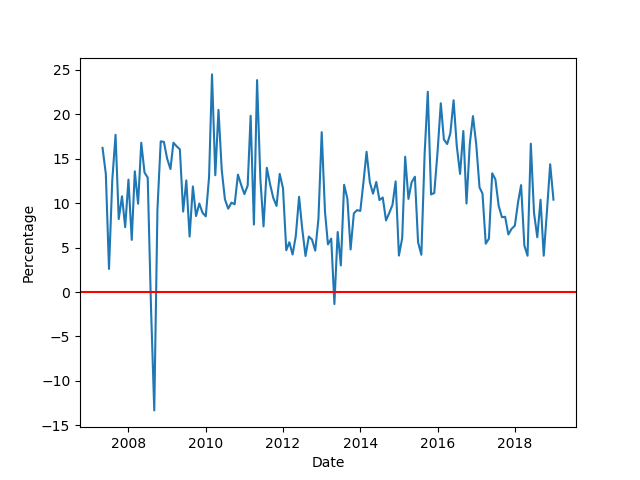
\includegraphics[scale=.75]{images/carryTrade/monthly1.png}
    \caption{Percentage Profit From Monthly Carry Trade (Weight = [100])}
    \label{simulationfigure}
\end{figure}

\begin{itemize}
  \item Average Percentage profit: 10.89
  \item The strategy makes the biggest loss around 2008, which was during the financial crisis.
  \item The biggest loss of the strategy is about 10 percentage point smaller than the biggest profit.
  \item In order to get rid of loss it might be a good idea to diversify our portfolio by assigning weights.
\end{itemize}

\begin{figure}[H]
    \centering
    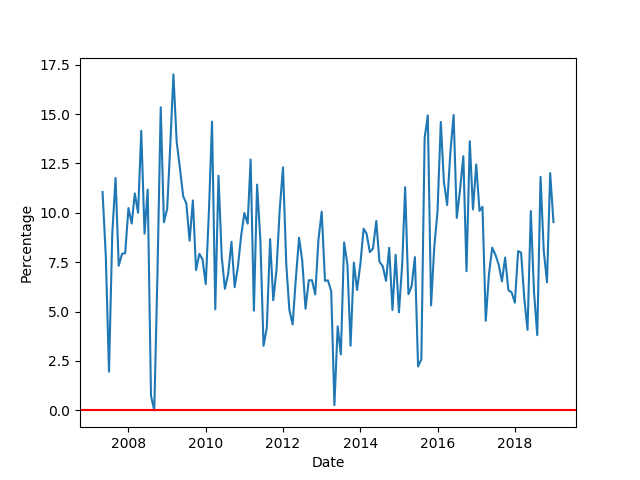
\includegraphics[scale=.75]{images/carryTrade/monthly2.png}
    \caption{Percentage Profit From Monthly Carry Trade (Weight = [40,30,30])}
    \label{simulationfigure}
\end{figure}

\begin{itemize}
  \item Average Percentage profit: 8.29
  \item Although our average profit reduced, our strategy does not face any major losses.
  \item Borrowing from multiple countries and lending to multiple countries has allowed us to reduce any potential risk and losses.
  \item A further step to this will be to come up with a dynamic system that automatically adjusts weights for short and long after every single trade.
  \item Another advancement that can be introduced is the use of dynamic trading intervals by allowing the algorithm to decide the best for going short and long.
\end{itemize}

\subsubsection{Return on Trading for Half Year(6 months) Basis}

\vspace*{-6.8mm}

\begin{figure}[H]
    \centering
    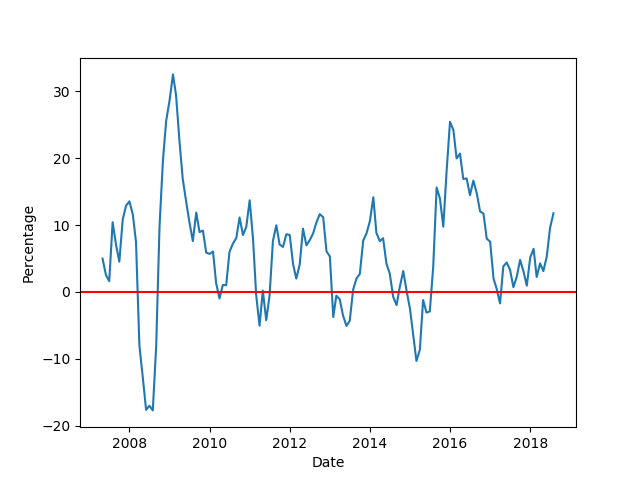
\includegraphics[scale=.75]{images/carryTrade/halfYear1.png}
    \caption{Percentage Profit From Half Year Carry Trade (Weight = [40,30,30])}
    \label{simulationfigure}
\end{figure}

\begin{itemize}
  \item Average Percentage profit: 6.17. (Lower than the monthly Average Percentage Return)
  \item The number of losses faced by the trading strategy increases as the trading interval increases from 1 month to 6 months.
  \item It appears to be more profitable and risk aversive to indulge in carry trade over monthly basis rather than half-year basis.
  \item This indicates that interest rate differential for carry trade is a more beneficial over shorter periods of time.
  \item UIP might come to hold over the long run making carry trade not profitable.
  \item Longer trade interval results in higher risk because half year is enough time for a country's economic situation to change.
  \item It will be interesting to see if introduction of dynamic weight portfolio optimization strategy will make carry trade also profitable over the long run.
\end{itemize}

% \begin{equation}
%     \label{simple_equation}
%     \alpha = \sqrt{ \beta }
% \end{equation}

\section{Predicting the Directional Change in Foreign Exchange Returns}

\subsection{Feature Engineering}

\vspace*{1mm}

\subsubsection{Monthly Exchange Rate Return}

\vspace*{2mm}

The equation below shows the exchange rate return that you gain if you go short on a currency one month after you bought it. This equation has been acquired from the following source:
https://www.investopedia.com/articles/forex/12/calculating-profits-and-losses-of-forex-trades.asp

\[return_t^i=\frac{er_t^i - er_{t+1}^i}{er_{t+1}^i}\]}

\begin{itemize}
  \item $\[er_t\]$ = is current exchange rate of a foreign currency (USD as base currency.)
  \item $\[er_{t+1}\]$ = one month ahead exchange rate of a foreign currency (USD as base currency.)
  \item superscript i indicates the country being considered
\end{itemize}


\begin{figure}[H]
    \centering
    \hspace*{-2.5in}
    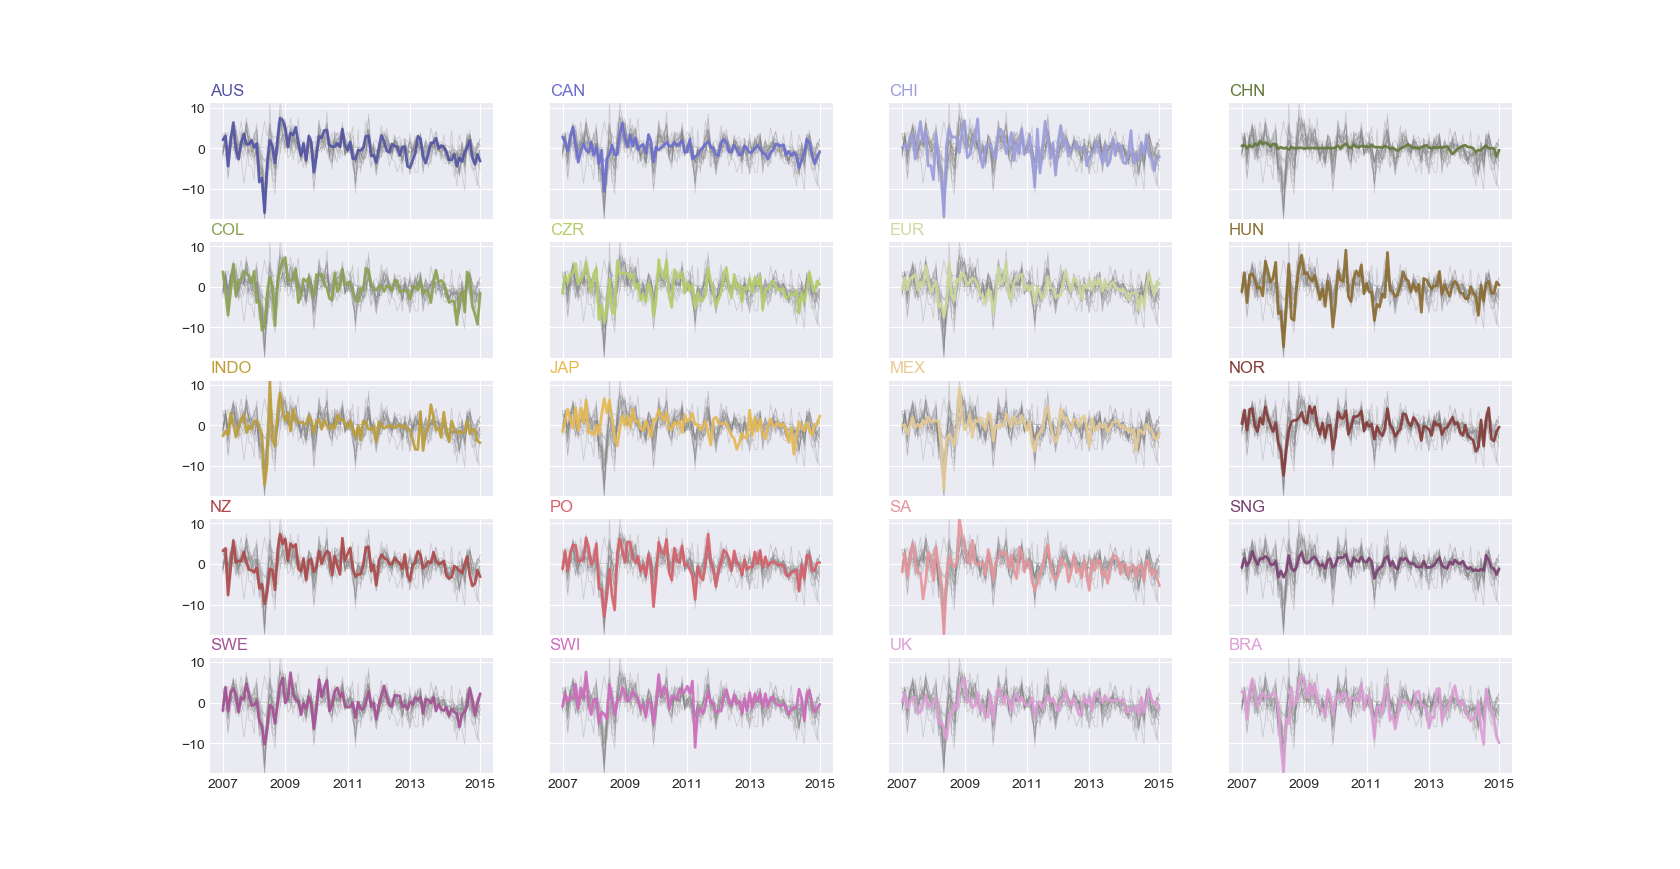
\includegraphics[scale = .58]{images/direction/er_return.png}
    \caption{Monthly Exchange Rate Return for all countries from 2007 to 2015}
    \label{simulationfigure}
\end{figure}

\begin{itemize}
  \item China appears to have the least volatility in exchange rate returns as their currency is pegged against USD.
  \item It is interesting to see how almost all currencies faced an instant fall in exchange rate returns during the 2008 financial crisis.
  \item Singapore appears to have the second least volatility in exchange rate returns after China.
\end{itemize}

\newpage

\subsubsection{Principal Component Analysis of Yield, Expectation and Term Premium}

\vspace*{5mm}

Our interest rate or yield data ranges from 2 months up until 120 months for each country. Similarly the term premium
and expectation component of yield curve also range from 2 months to 120 months for each country. In order to account for
all short and long term yield and its component's data, I take the first three principal components of all three variables for all countries.
On average the first three PCA describes more than 95 percent variance of all the variables. According to theory the first three principal components
of yield, expectation, and term premium account for the level, slope and curative of the variables respectively. The following nine variables were generated
after PCA:

\vspace*{5mm}
\begin{itemize}
  \item yield level
  \item yield slope
  \item yield curvature
  \item expectation level
  \item expectation slope
  \item expectation curvature
  \item term premium level
  \item term premium slope
  \item term premium curvature
\end{itemize}


\begin{figure}[H]
    \centering
    \hspace*{-2.5in}
    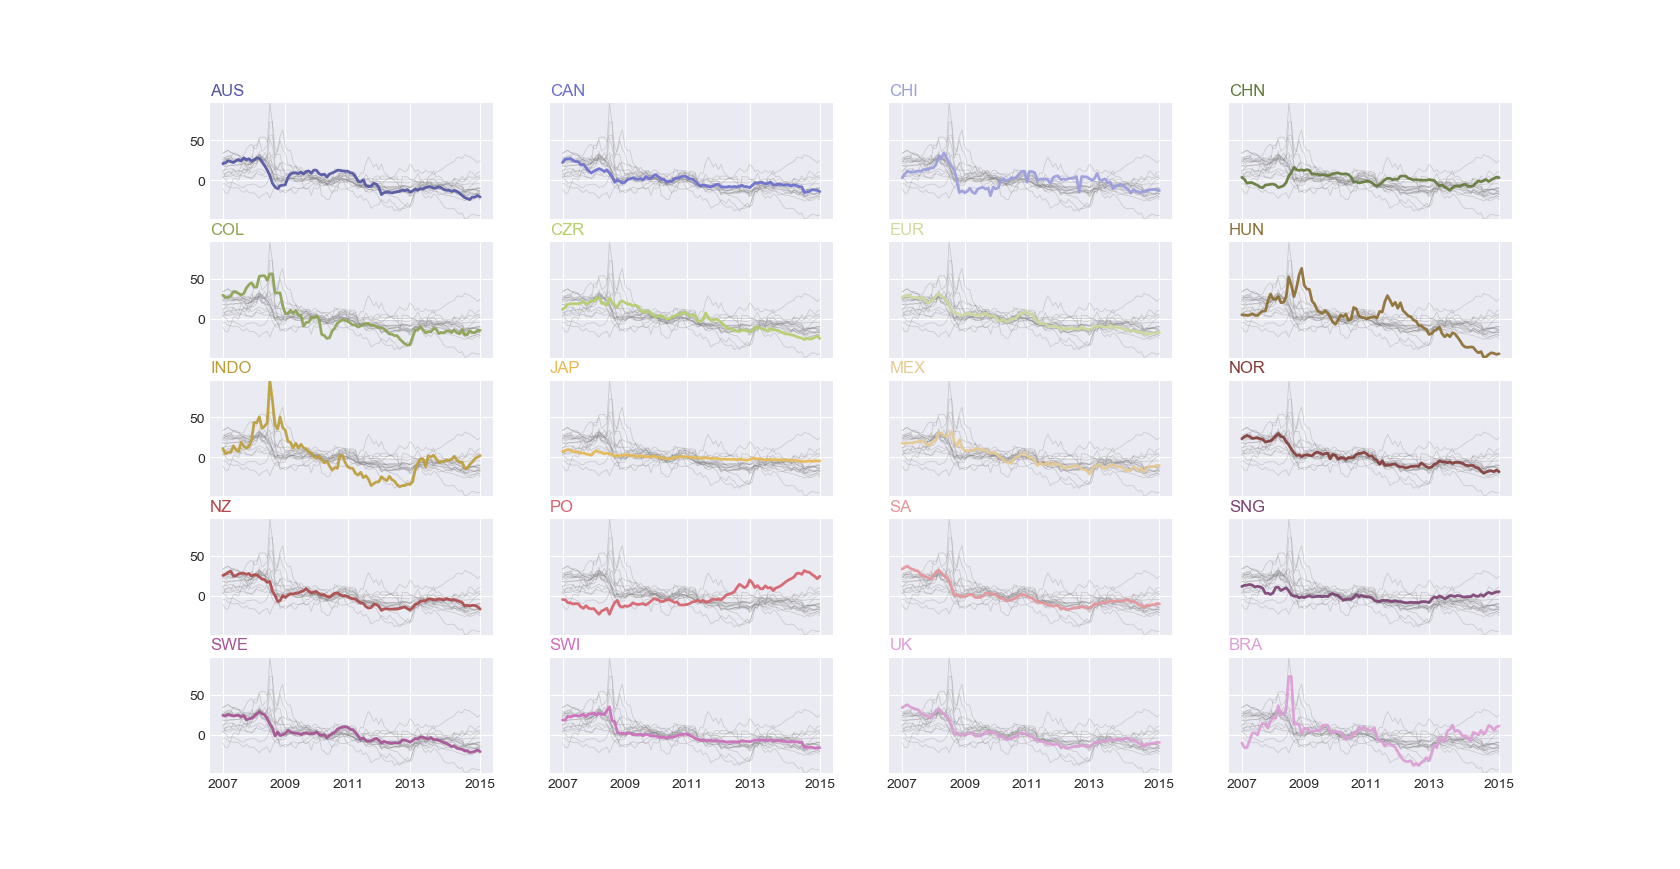
\includegraphics[scale = .58]{images/direction/yield_level.png}
    \caption{Yield Level for all countries from 2007 to 2015}
    \label{simulationfigure}
\end{figure}

\begin{figure}[H]
    \centering
    \hspace*{-2.5in}
    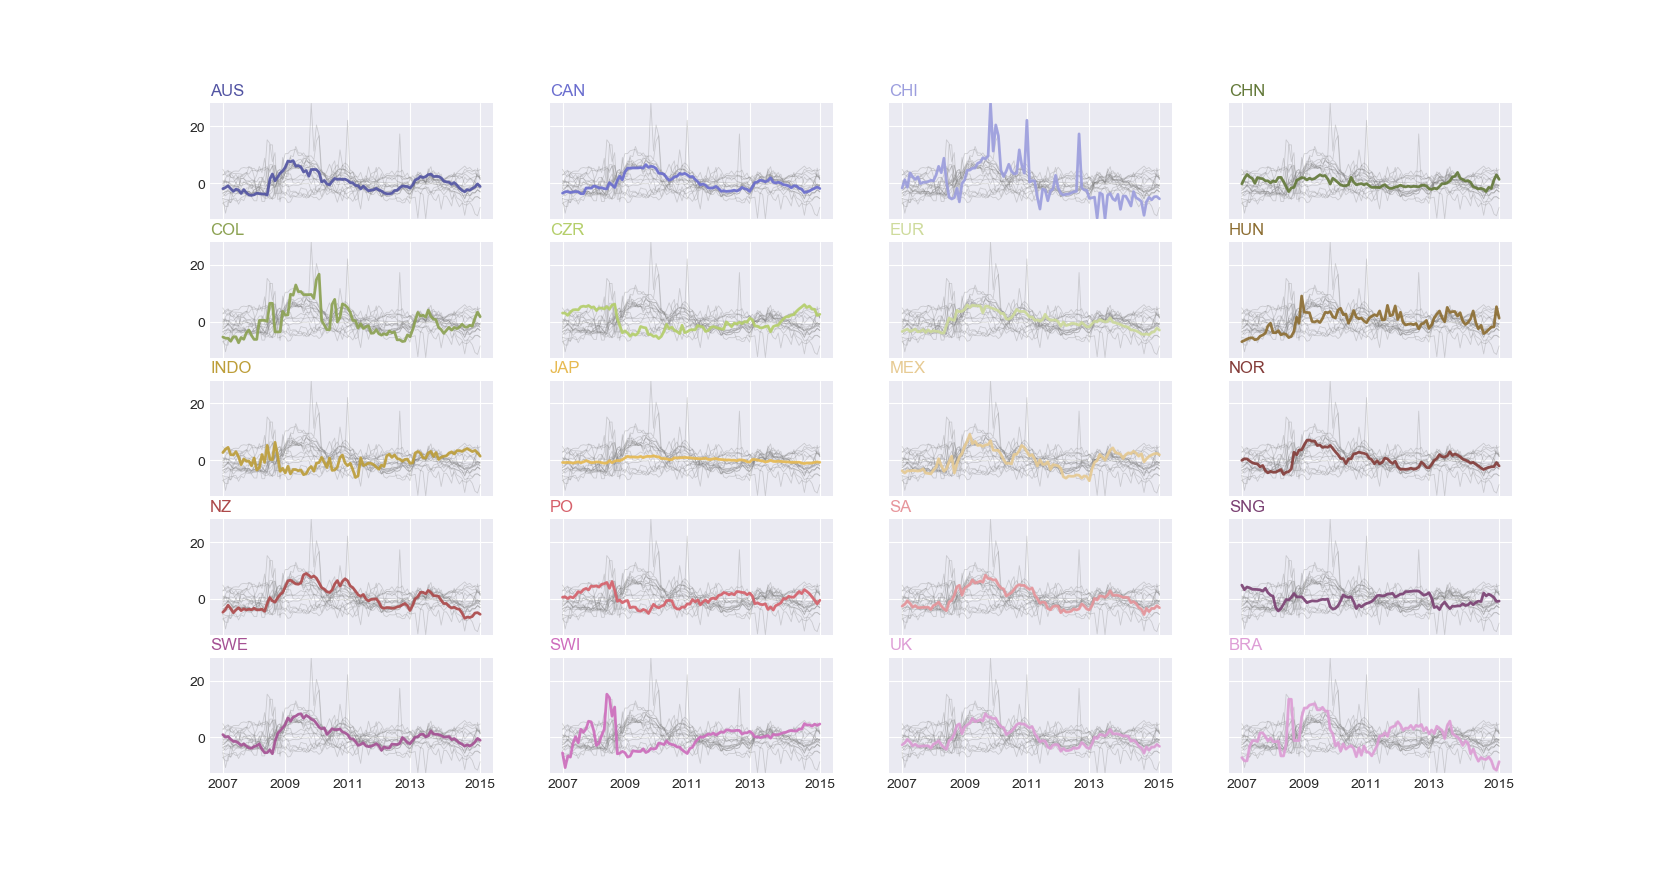
\includegraphics[scale = .58]{images/direction/yield_slope.png}
    \caption{Yield Slope for all countries from 2007 to 2015}
    \label{simulationfigure}
\end{figure}

\begin{figure}[H]
    \centering
    \hspace*{-2.5in}
    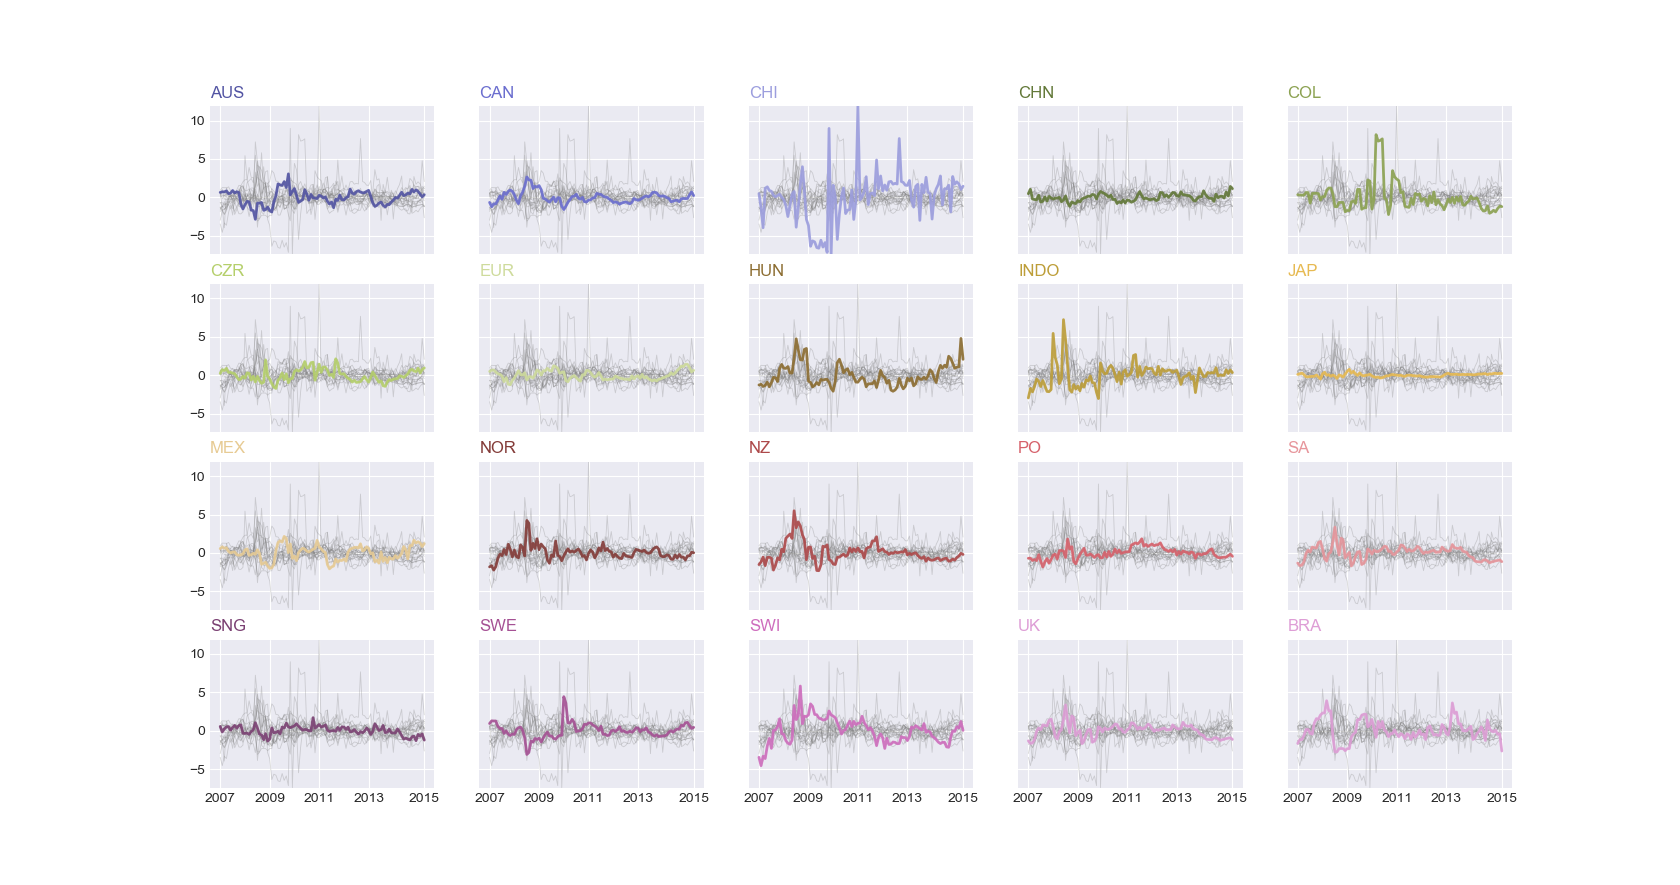
\includegraphics[scale = .58]{images/direction/yield_curvature.png}
    \caption{Yield Curvature for all countries from 2007 to 2015}
    \label{simulationfigure}
\end{figure}

\begin{itemize}
  \item China appears to be the most stable across all three components of yield.
  \item It is interesting to see how Chile appears relatively normal in yield level but faces drastically increased volatility in the slope and curvature component.
  \item Similar graphs for the expectation and term premium components were also created which can be included in the appendix.
\end{itemize}

\newpage

\subsection{Support Vector Machine for Buy/Sell Classification}
\vspace*{5mm}

\subsubsection{Setup}

\vspace*{5mm}

\begin{itemize}
  \item A 70/30 percent train/test split was created to check in and out of sample performance of our model.
  \item A binary column named "buy" was created which was given a value of 1 for one month ahead positive return and a 0 for one month ahead negative or zero return.
  \item A machine learning technique called Grid Search was used to find the best parameters for our support vector classifier. Grid Search fits model with different
  parameters and uses cross validation to find the best combination.
  \item Support Vector Classification Models were for all countries, and confusion matrix on the train and test datasets were used to check the performance of our models.
\end{itemize}

\begin{figure}[H]
    \centering
    \hspace*{-1.25in}
    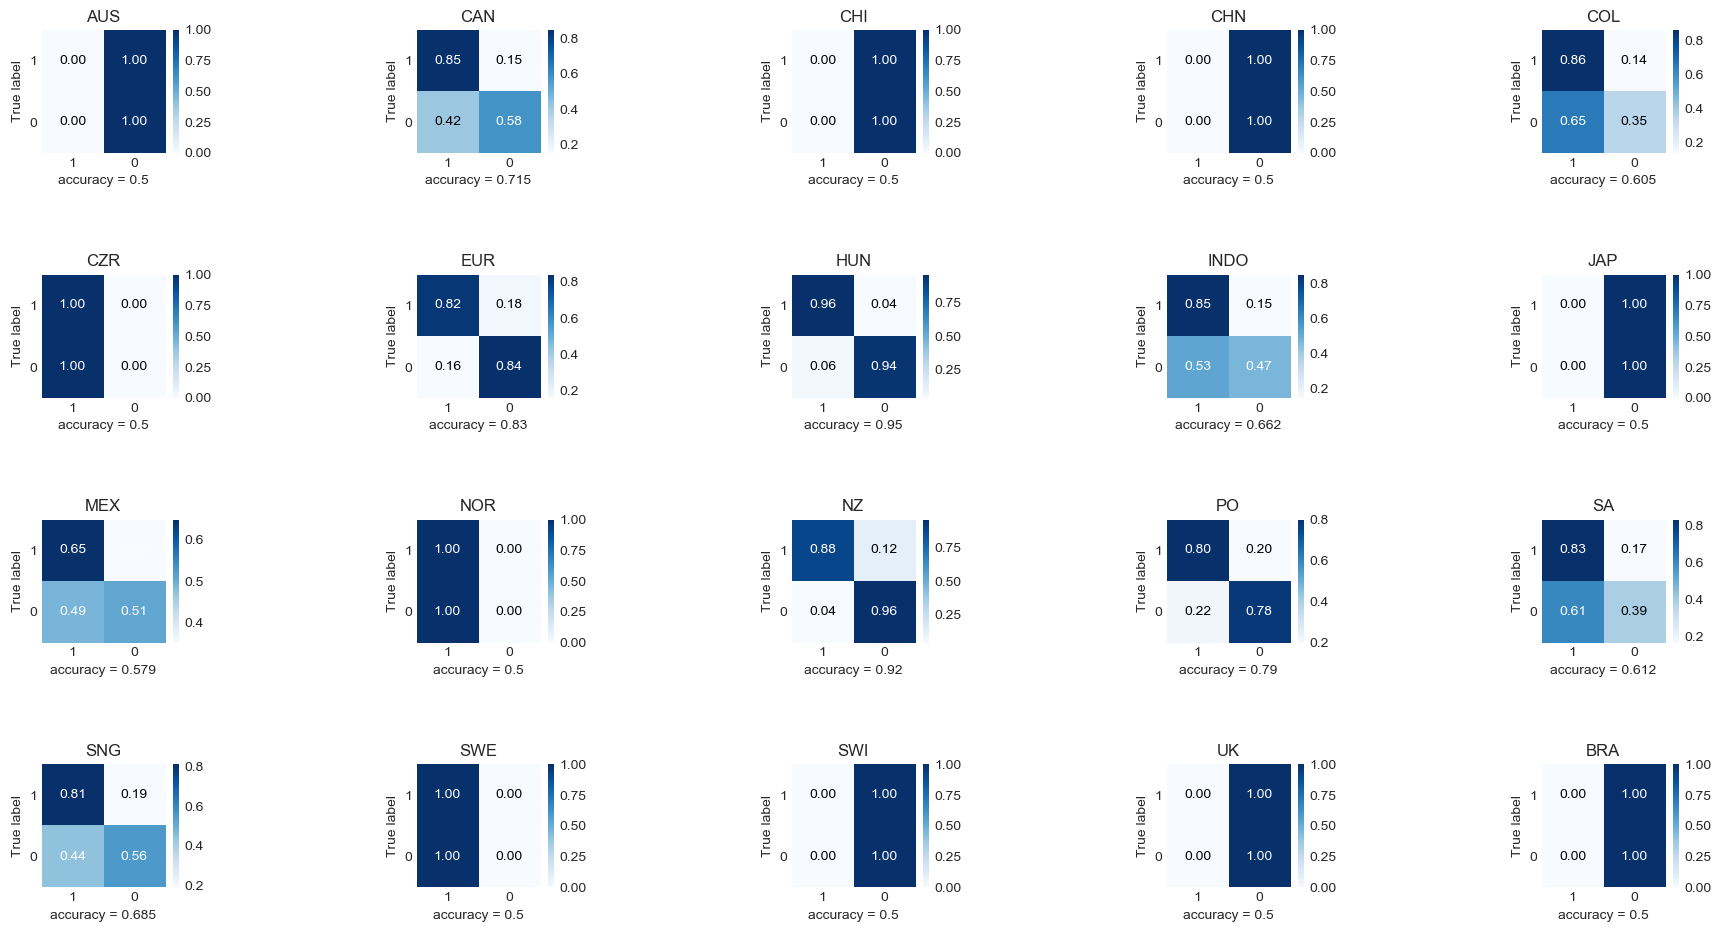
\includegraphics[scale = .30]{images/direction/clf_cm_train.png}
    \caption{SVC Confusion Matrix for all countries for Training Dataset}
    \label{simulationfigure}
\end{figure}

\begin{figure}[H]
    \centering
    \hspace*{-1.25in}
    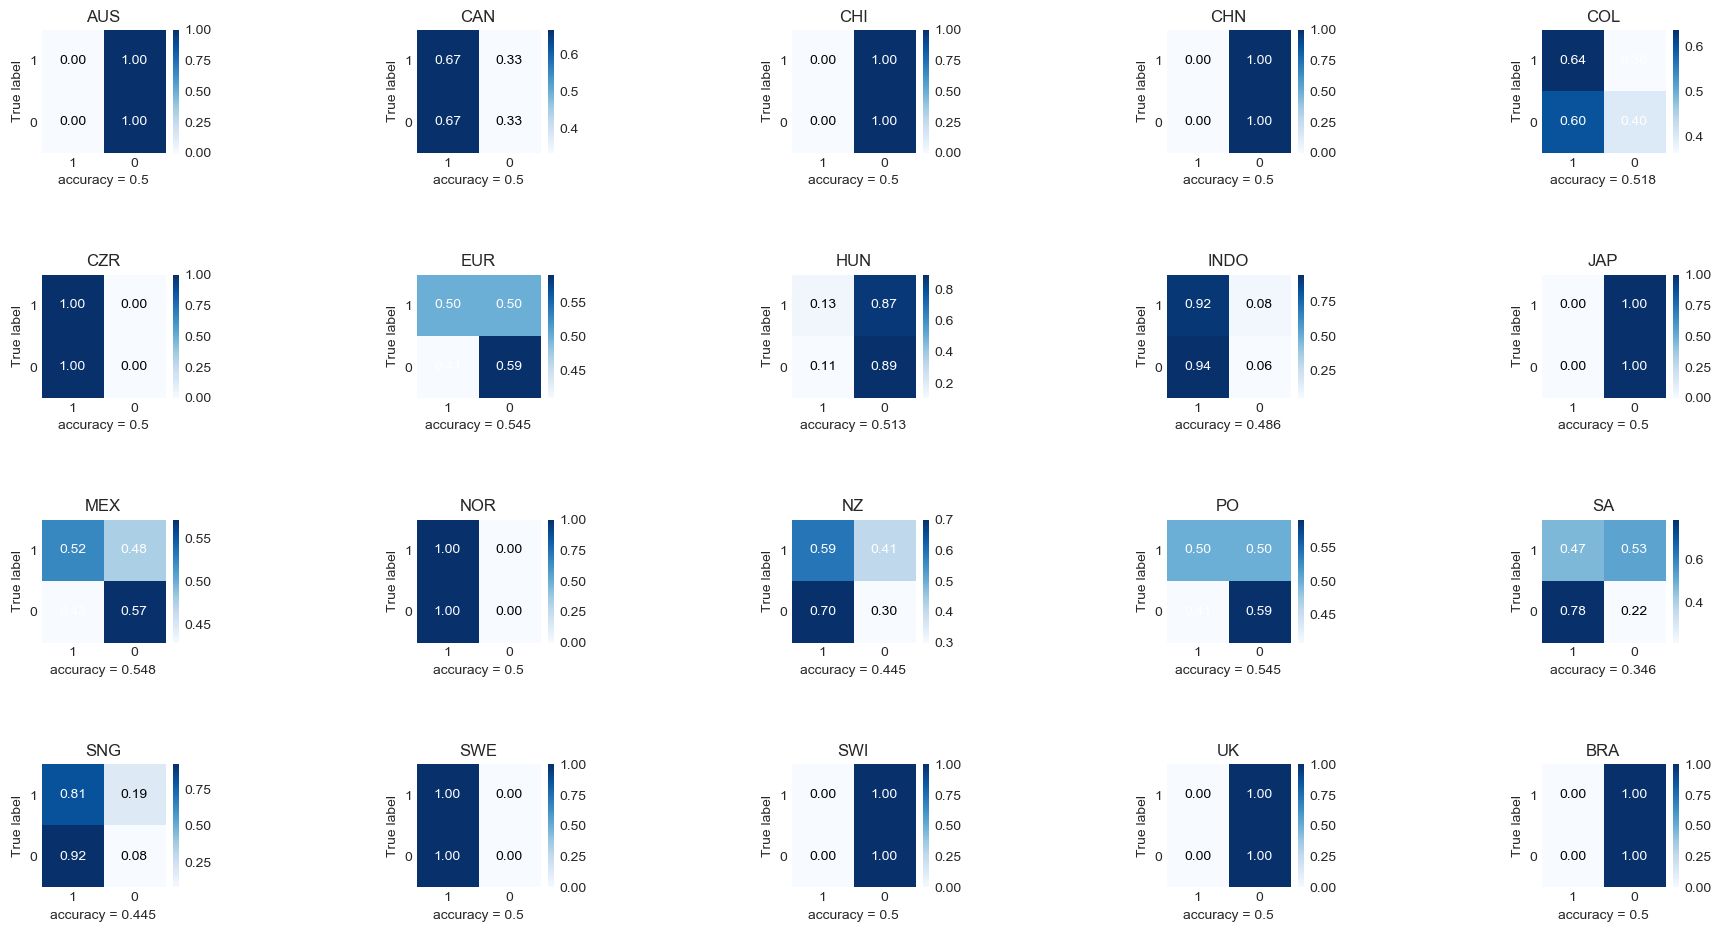
\includegraphics[scale = .30]{images/direction/clf_cm_test.png}
    \caption{SVC Confusion Matrix for all countries for Test Dataset}
    \label{simulationfigure}
\end{figure}

\begin{itemize}
  \item On training dataset most country's models seem to perform better than random walk model (random guess).
  \item On test dataset only a few country's model perform better than random walk, while others being similar to worse than random walk.
  \item It appears that most models created are not generalizable as their in sample performance is way better than their out of sample performance.
  \item It would be interesting to add sentiment and uncertainty variables extracted from FOREX news to the model as they might significantly improve the performance
        of the model as their is a general hypothesis that news articles dictate foreign exchange directional change over the long run.
\end{itemize}


\subsection{Neural Network for Buy/Sell Classification}
\vspace*{5mm}

\subsubsection{Setup}

\vspace*{5mm}

\begin{itemize}
  \item A multi-layer perceptron with 2 hidden layer is created.
  \item The first hidden layer consists of 64 nodes, while the second hidden layer consists of 32 nodes.
  \item RELU activation function is used in the first two layers (best for classification task according to literature) and sigmoid activation function is used in the output
        layer for binary classification.
  \item 1000 epochs were run for each model to repetitively improve the model using back propagation.
  \item Neural Network Models were for all countries, and confusion matrix on the train and test datasets were used to check the performance of our models.
\end{itemize}

\begin{figure}[H]
    \centering
    \hspace*{-1.25in}
    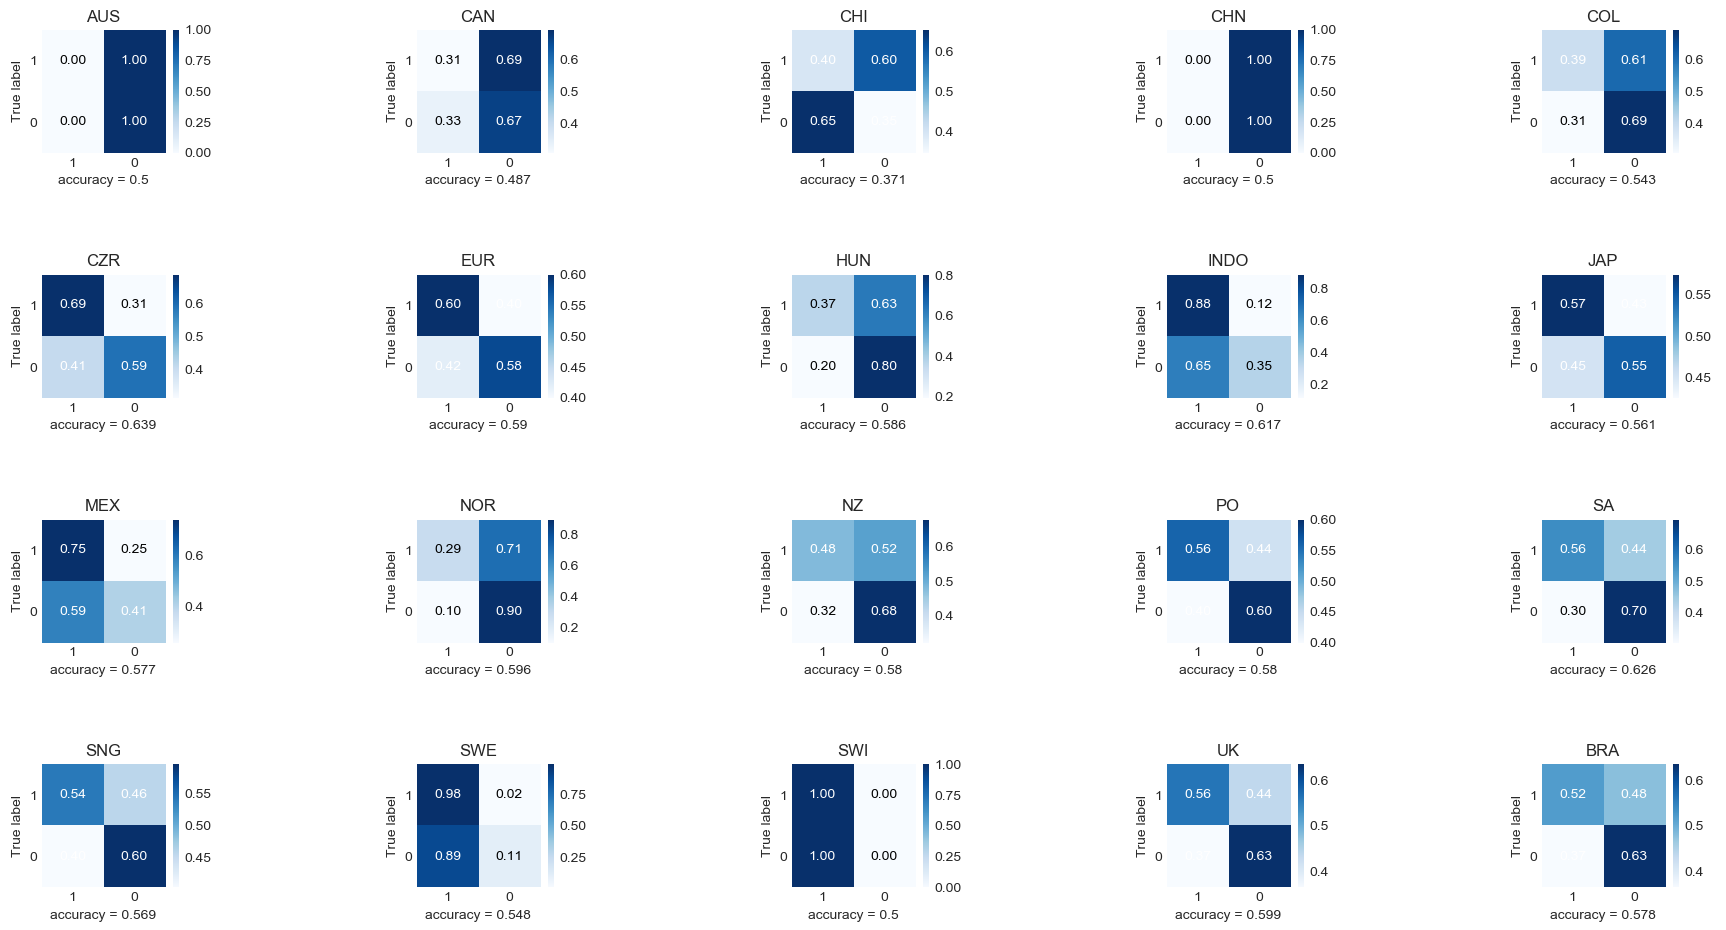
\includegraphics[scale = .30]{images/direction/n_cm_train.png}
    \caption{Neural Network Confusion Matrix for all countries for Training Dataset}
    \label{simulationfigure}
\end{figure}

\begin{figure}[H]
    \centering
    \hspace*{-1.25in}
    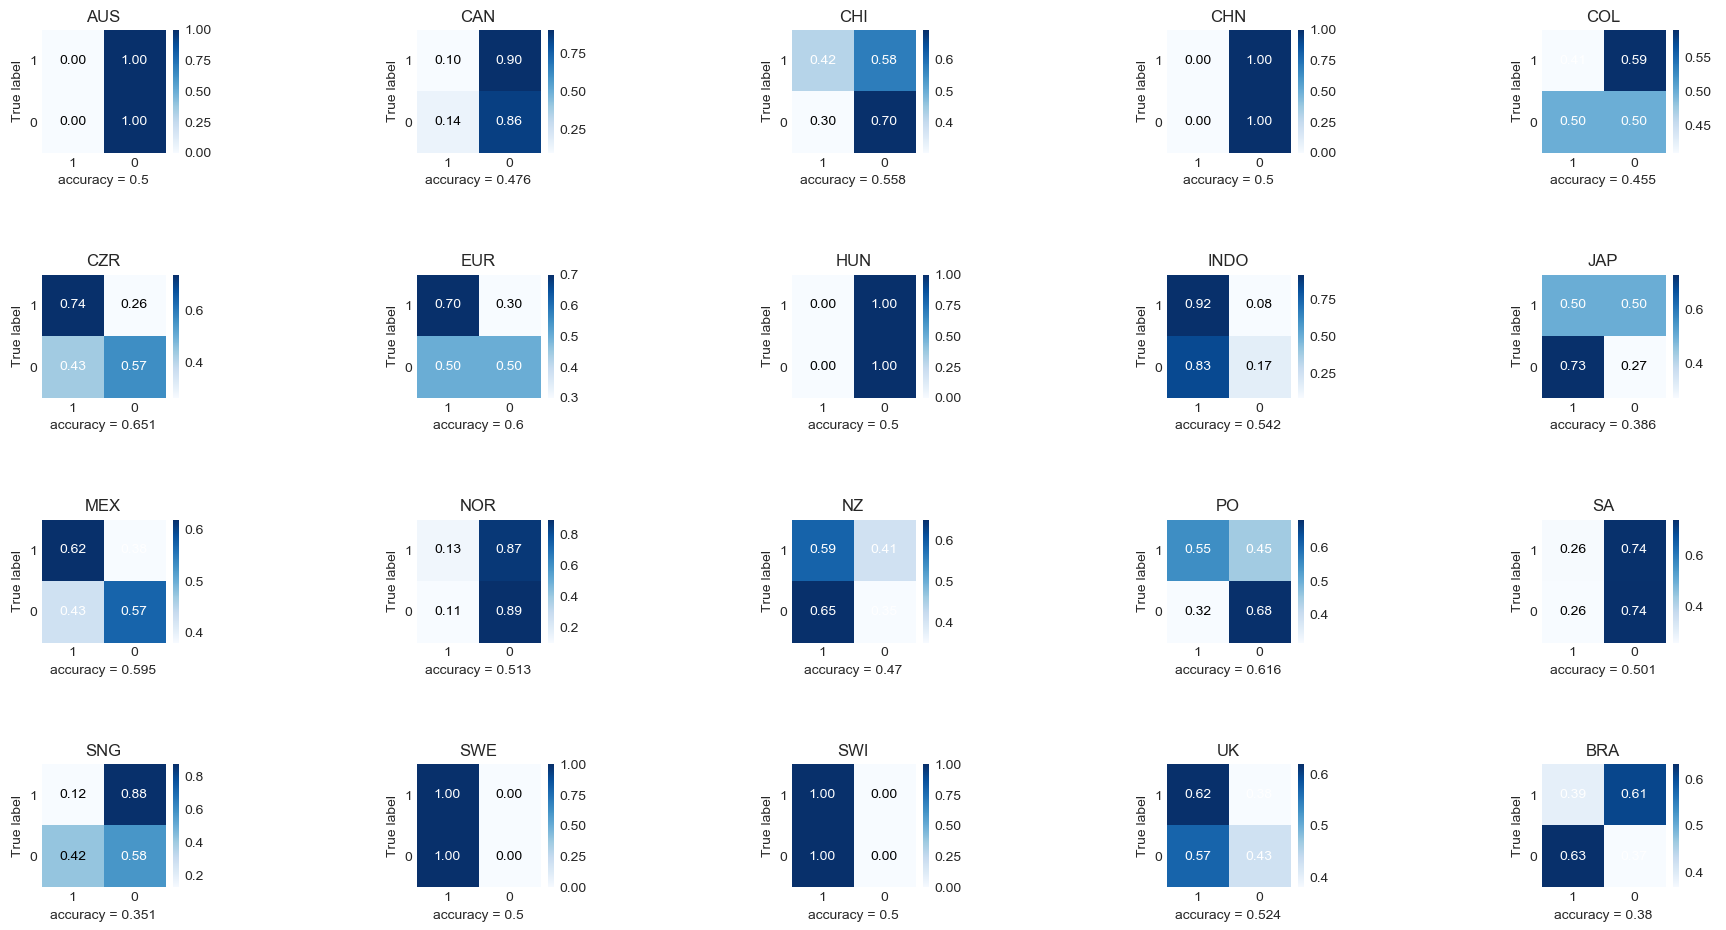
\includegraphics[scale = .30]{images/direction/n_cm_test.png}
    \caption{Neural Network Confusion Matrix for all countries for Test Dataset}
    \label{simulationfigure}
\end{figure}

\begin{itemize}
  \item On training dataset most country's models seem to perform better than random walk model (random guess).
  \item Unlike SVC, on test dataset most countries model still tend to perform better or equal to that of random walk.
  \item It appears that our neural network classifier is more generalizable than our SVC classifier. Although it only manages to beat the random walk in a few cases and be mostly
        equal in others.
  \item It would be interesting to add sentiment and uncertainty variables extracted from FOREX news to the model as they might significantly improve the performance
        of the model as their is a general hypothesis that news articles dictate foreign exchange directional change over the long run. Neural Networks will improve more
        than SVC with sentiment data as deep learning techniques perform better than machine learning technqiues with huge datasets.
\end{itemize}

\section{Predicting Directional Change in FOREX market with Sentiment Analysis}
\vspace*{2mm}

\subsection{Variables of Interest}
\subsubsection{Macro Variables}

\vspace*{2mm}

\[{\Delta}er_t^i=\frac{er_t^i - er_{t-1}^i}{er_{t-1}^i}\]}

\begin{itemize}
  \item $\[\Delta}er_t^i\]$ represents the change in daily exchange rate at time 't'.
  \item $\[er_t^i\]$ represents the exchange rate of a country at time 't'.
  \item $\[er_{t-1}^i\]$ represents the historical exchange rate of a country at time 't-1'.
  \item Superscript i indicates the country being considered.
  \item All currencies have USD as its base currency.
  \item 't' indicates daily exchange rate data from 2009 to 2019.

\end{itemize}

\[interest\: rate\: diff_t^i= US\:interest\:rate_t - foreign\: interest\: rate_t^i}

\vspace*{2mm}

\begin{itemize}
  \item $\[interest\: rate\: diff_t^i$ represents daily US interest rate difference with a foreign country 'i' at time 't'.
  \item 't' indicates daily interest rate data from 2009 to 2019.
  \item 'i' subscript indicates the country being considered.
  \item The list of countries being considered are [AUS ,  CAN ,  CHI ,  CHN ,  COL ,  CZR ,  EUR ,  HUN ,
                       INDO ,  JAP ,  MEX ,  NOR ,  NZ ,  PO , SA ,  SNG , SWE ,  SWI ,  UK  , BRA]
\end{itemize}
\newpage

\subsubsection{Textual Data}
\vspace*{2mm}

All textual data, in the form of foreign exchange rate news articles, has been collected from investing.com's FOREX section. The dataset contains all exchange rates related
news articles that has been published from 2009 to 2019. The dataset consists of 82,500 FOREX news articles.

\begin{figure}[H]
    \centering
    %\hspace*{2.5in}
    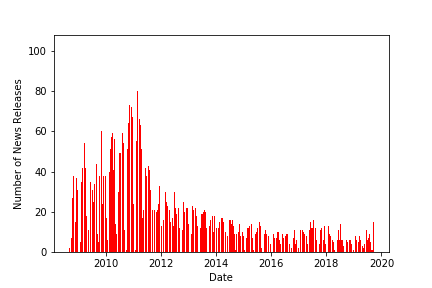
\includegraphics[scale = .80]{images/sentiment_analysis/news_frequency.png}
    \caption{Daily FOREX News Release Frequency on Investing.com}
    \label{simulationfigure}
\end{figure}

\begin{itemize}
  \item The figure above shows daily news release frequency on Investing.com from 2009 to 2019.

  \item The daily news frequency appears to increase significantly from 2009 to 2011. This might be a result of the increase in financial and economic uncertainty caused by the 2008 recession.

  \item After around 2012, the number of FOREX news article releases appear to average out at around 20 per day.

  \item The daily number of news releases may be expected to increase after 2016 because of Brexit. However, this does not appear to be the case in the figure above as the number of news releases has less variation after 2014. This may be a result of a drop in business for investing.com after 2012. With the introduction of Bloomberg and other advanced financial news sources, the demand for investing.com news articles may also have gone down, leading to a reduction in their daily news article releases.
\end{itemize}

\subsection{Text Preprocessing}

In order to use our textual data for sentiment analysis, we will need to clean it and convert it into vector format. It is important for us to clean up our dataset in order to eliminate any noise that might influence our analysis. Computers can only understand data in vector format. Hence, after the text cleaning process, we will need to convert the remaining dataset into vector format using various techniques such as bag of words or TF-IDF vectorization. Only after we have converting our data into vector format can we feed it into our algorithms to get useful insight. This process of text cleaning and text to vector conversion is known as text preprocessing.


\subsubsection{Text cleaning}
Natural language processing is both a time and memory consuming process. Cleaning textual data before converting it into vectors reduces run time. It also helps us avoid extra memory allocation by getting rid of content that might introduce noise in the dataset. This helps focus on content that is most relevant to our analysis. Text cleaning takes place in the following order:

\begin{itemize}
  \item \emph{Removing the HTML Tags:} The textual data contains HTML tags because the dataset was scraped from investing.com (eg: $<p>$, $<h2>$ etc). HTML tags do not add any meaning to the dataset during the analysis. It is important to get rid of them in order to eliminiate noise into the dataset.

  \item \emph{Removing Punctuations:} Similar to HTML tags, punctuation adds unnecessary extra detail. Hence it is a good idea to eliminate it in order to save memory space and computation time.

  \item \emph{Removing Stop words:} Stop words like 'this', 'there', 'is', 'make' etc can also be unnecessary. However, it is important to be cautious while getting rid of stop words such as 'not'. While, it is considered a stop word in many Python libraries (including sPacy), it can be critical to interpreting data.

  \item \emph{Stemming:} This is the process of extracting root words from a text. Words like 'tasteful', 'tastefully' etc are all variations of the word 'tasty'. Instead of having to create a vector for each of these words, it is better to stem all the words to their root as it helps to better analyze and interpret the textual dataset.

  \item \emph{Lemmatization:} Similar to stemming, lemmatization is used to convert a word back to its base form. However, this process uses a dictionary for vocabulary and morphological analysis of words. While stemming processes words individually, lemmatization also considers the context in which it is being used. Lemmatization, for example, can identify that 'good' is the base form of 'better' while stemming will not account for this.

  \item \emph{Converting everything to lower case:} Words like 'Biscuit' and 'biscuit' are classified differently because computers cannot differentiate between the uppercase and lowercase form of a word. For this reason, it is important to convert all textual data to lower case form in order to enhance model performance.

\end{itemize}

\subsubsection{Text to vector conversion}
Next, we will need to convert the dataset into vector form. There are multiple techniques that can be used to project text onto a vector space. The three techniques used in this paper are:

\begin{itemize}

  \item \emph{Bags of Words:} This is the simplest method for projecting text onto a vector space. This technique creates a dictionary of 'n' words where 'n' is the number of unique words in our text corpus. It then creates an 'n' dimensional vector for each of our documents in the dataset. Each cell (or dimension) in the bag of words has a value representing the number of times the corresponding word has occurred in the document. As the vocabulary of the whole dataset increases, the number of dimensions in the bag of words also increases. This means that for each document in a big dataset the number of zeros will exceed the number of non zeros. Vectors where the majority of values are zeros are referred to as \emph{sparse vectors}. Many sparse vectors stacked on top of each other create a grouping are called a \emph{sparse matrix}.

  \item \emph{Term Frequency-Inverse Document Frequency (TF-IDF):} This is a more advanced text to vector conversion technique that contains two concepts: Term Frequency (TF) and Inverse Document Frequency (IDF). Term Frequency (TF) refers to the frequency of a word appearing in a document. TF aims to identify words that are most occurring in a document. It can be represented as:

\[TF=\frac{Number \: of \: time \: word \: appear \: in \: the \: document}{Total \: number \: of \: words \: in \: the \: document}\]}

Inverse Document Frequency(IDF), on the other hand, aims to find the importance of a word by checking its uniqueness across the complete dataset. IDF is based on the idea that words that are less frequent across the documents but frequent within a specific document are critical to understanding the document.

\[IDF=log_{10}\frac{Total \: number \: of \: documents}{Number \: of \: documents \: in \: which \: word \: appears}\]}

TF-IDF is a multiplication of the TF and IDF equations. It aims to identify the words that are unique to a specific document in order to better understand the content of a text. Multiplication of TF with IDF helps reduce the values for high frequency common words that occur across most of the dataset. It is a powerful technique that can be used for classifying text with different writing styles because it can identify words that are unique to a document.

  \item \emph{Word2Vec:} This is the most advanced and time consuming text to vector conversion technique among Bags of Words and TF-IDF. Word2Vec consists of all the deep learning models that can be used for generating \emph{word embedding}. A word embedding is an approach for providing a dense vector representation to a set of words that captures something about their meaning. The vector space representation of the words provide a projection where words with similar meanings are clustered together. These models consist of a shallow two layer neural network with one input layer, one hidden layer and one output layer. It is through the use of these pre-trained neural networks that we can generate word embeddings for textual data. The two main architectures utilized by Word2Vec models are \emph{CBOW}(Continous Bag of Words) and \emph{Skip Gram}. It is through the use of these word embedding techniques over other word to vector conversion techniques that has lead to breakthrough performance with deep neural networks on problems such as machine translation.


\end{itemize}

\newpage

\subsection{Sorting Text as Per Country}

\subsubsection{Process Explanation}

After preprocessing the foreign exchange news articles, it is important for us to sort them as per country in order to run sentiment analysis for country specific exchange rate (with USD as its base currency). The list of countries that are being considered are Australia, Canada, Chile, China, Colombia, Czech Republic, Hungary, Indonesia, Japan, Mexico, Norway, New Zealand, Poland, South Africa, Singapore, Sweden, Switzerland, United Kingdoms and Brazil. Our dataset contains about 82,500 news articles. It would be very time consuming (and almost impossible) for one to manually go through all the articles and group them by country. For this reason, I developed a sorting mechanism searches for specific country related words in a document along with word embedding and cosine similarity to incorporate any country specific words that might otherwise have been left out otherwise. A combination of straight forward searching and cosine similarity based searching is used to optimize sorting efficiency. Both the techniques are explained below:

\begin{itemize}

  \item \emph{Search for specific country related terms:} This method involves searching through all the documents in the dataset for country specific search terms. To do this, I first developed a specific list of search terms for each country with the following format: $[country\: name, currency\: code, citizenship]$. Every country had these three words in their list of search terms. For example, in case of Australia the search terms were $[australia, aud, australian]$. Afterwards, every document in the dataset was looped over in order to find each country's list of search terms. Every document was classified into different countries based on the search terms it contained. Finally, all the results were organized into separate news article data frames for each country.

  \item \emph{Search based on cosine similarity:} Simply searching for specific search terms to classify data is not the most effective way to sort textual data by country because their always remains a possibility that we might be missing some country specific search terms that are important for grouping our news articles. This means that there is always a chance of miscategorizing. In order to minimize the probability of miscategorizing valuable news articles, I combine the searching process with a text similarity technique called cosine similarity. \emph{Text similarity} is the process of determining how 'close' two pieces of text are, both in lexical (surface closeness) and semantic (meaning) similarity. These techniques make use of word embedding to represent documents in multi-dimensional vector space and compare documents by measuring the distance between the vectors in the feature space. Cosine similarity is one of the most widely used methods for text similarity. It calculates the similarity between texts by measuring the cosine of the angle between two vectors. The cosine similarity index ranges from 0 to 1 where 0 indicates the least similar, while 1 indicates perfect similarity. It is beneficial to use this technique while sorting data by country because it enables to catch any country specific terms that might have been missed. For example words like 'Toronto' and 'Ontario' have more than 0.5 cosine similarity with 'Canada'. This means we can simply use a country name along with cosine similarity to search for all articles relating to it. In order to apply the technique based on cosine similarity, each document in the dataset was projected on a vector space using Word2Vec. Afterwards, the same country specific search terms used in previous searching methods were also projected onto a vector space. Finally, any document containing text that had a cosine similarity of more than 0.5 with a specific country's search term was classified accordingly. All results were organized into country specific data frames.

  \item \emph{Combining both search results:} Once individual news article data frames for each country were created, using both simple and cosine similarity searching methodologies, the results from both models where combined into a bigger dataset for each specific country. In the case where each of the two strategies classified the same document to one country, the resultant dataset will contain duplicate content. In order to prevent any duplication in the final datasets for each country, observations that occurred more than once in the dataset were eliminated.

\end{itemize}

\newpage

\subsubsection{Textual Data Structure}

The following table shows the length of country specific news article datasets that were created after combining the results of simple and cosine similarity searching methodologies:

\vspace*{6mm}

\begin{tabular}{ |p{3cm}||p{3cm}|p{3cm}|p{3cm}|  }
 \hline
 \multicolumn{2}{|c|}{Dataset Lengths} \\
 \hline
 Country Code & Number of articles\\
 \hline
 AUS   & 26074\\
 CAN   & 30591\\
 CHI   & 331\\
 CHN   & 15634\\
 COL   & 3978\\
 CZR   & 1297\\
 EUR   & 64807\\
 HUN   & 1183\\
 INDO  & 1024\\
 JAP   & 38023\\
 MEX   & 2365\\
 NOR   & 641\\
 NZ    & 14524\\
 PO    & 929\\
 SA    & 5515\\
 SNG   & 8618\\
 SWE   & 1211\\
 SWI   & 17158\\
 UK    & 34530\\
 BRA   & 1791\\
 \hline
\end{tabular}
\vspace*{8mm}

According to the results of sorting news articles by country/currency, the Euro appears to have the largest number of articles, followed by Japan and then the United Kingdoms. Chile, on the other hand, appears to have the least amount of FOREX news articles, followed by Norway and then Poland. This shows that most of the articles on investing.com focus on the exchange rate of many European countries, Canada, Japan and China.

\vspace*{8mm}
\newpage
Machine learning and deep learning techniques for textual analysis perform better on bigger datasets. The performance of a machine learning model is directly proportional to the size of its training dataset. This is because large datasets consist of more observations that can be used to train models. In order to make sure that the models for each country has enough training datasets, I decide to get rid of any country that has less than 3000 articles. This leaves us with the following 11 countries for further analysis:

\vspace*{6mm}


\begin{tabular}{ |p{3cm}||p{3cm}|p{3cm}|p{3cm}|  }
 \hline
 \multicolumn{2}{|c|}{Dataset Lengths} \\
 \hline
 Country Code & Number of articles\\
 \hline
 AUS   & 26074\\
 CAN   & 30591\\
 CHN   & 15634\\
 COL   & 3978\\
 EUR   & 64807\\
 JAP   & 38023\\
 NZ    & 14524\\
 SA    & 5515\\
 SNG   & 8618\\
 SWI   & 17158\\
 UK    & 34530\\
 \hline
\end{tabular}

\subsubsection{Effectiveness of news articles distribution}

In order to check for the effectiveness of the textual distribution among countries, I make use of word clouds to visualize the most frequently used words in each country's dataset. Ideally, every country's word cloud should have words relating to different economic and financial components of the country. The extent to which we can distinguish between the word clouds of each country determines the effectiveness of our sorting mechanism. More distinguishable word clouds indicate effective performance of our sorting algorithm.

\begin{figure}[H]
    \centering
    %\hspace*{2.5in}
    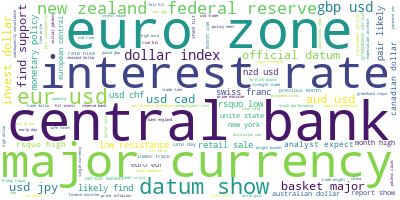
\includegraphics[scale = .58]{images/sentiment_analysis/CAN_wordCloud.png}
    \caption{Word Cloud for Canada representing Top 100 words}
    \label{simulationfigure}
\end{figure}

\begin{figure}[H]
    \centering
    %\hspace*{2.5in}
    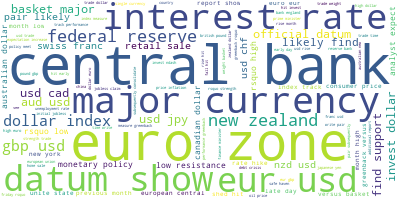
\includegraphics[scale = .58]{images/sentiment_analysis/CHN_wordCloud.png}
    \caption{Word Cloud for China representing Top 100 words}
    \label{simulationfigure}
\end{figure}

\begin{figure}[H]
    \centering
    %\hspace*{2.5in}
    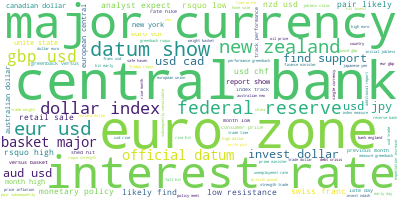
\includegraphics[scale = .58]{images/sentiment_analysis/JAP_wordCloud.png}
    \caption{Word Cloud for Japan representing Top 100 words}
    \label{simulationfigure}
\end{figure}

\begin{itemize}
  \item Although word clouds for all eleven countries in the dataset were created, the figure above shows word clouds for only Canada, China, and Japan respectively (these country's word clouds should ideally differ more.)
  \item Unfortunately, the word clouds for China, Canada and Japan do not appear to vary greatly. This indicates that our sorting mechanism was not as efficient as expected. It is understandable that 'interest rate' was the most frequent term in all three word clouds but it is unexpected that 'Euro Zone' is one of the most frequent words in China's and Japan's dataset.
  \item Every country's word cloud not only appears to have a mention of its own currency but also that of other country's currencies. This will lead to the introduction of noise in our textual datasets which causes our algorithm to misassociate one country's sentiment with that of another.
  \item The word clouds above show that our strategy for sorting text by countries was not very effective. This can influence our sentiment analysis results as our datasets might not be representative of the countries being considered.
  \item It will be vital to reconsider our text sorting mechanism if the exchange rate directional forecasting results with textual data are not significant.

\end{itemize}

\subsection{Sentiment Analysis}
Sentiment Analysis is a sub field of Natural Language Processing that aims to determine whether a piece of text is negative, positive or neutral in tone. This is also known as \emph{opinion mining} or \emph{emotion AI}. Sentiment Analysis helps us convert unstructured textual data into structured data that can then be used to train our models. Sentiment analysis is widely used in asset pricing and financial market analysis because of the importance of the expectation component in predicting different financial variables such as exchange rates and stock prices. News articles and social media are hypothesized to be the major driver of expectation in the economy. Machine learning algorithms cannot directly understand the text in a news or social media article. They require sentiment analysis or some other similar natural language processing technique to covert data into a processable format. Sentiment analysis informs us about the polarity of a news paper article which can be used to determine the directional change in exchange rate or any other asset price. Sentiment Analysis can be applied at different scope levels:

\begin{itemize}
  \item \emph{Document Level} sentiment analysis aims to obtain the sentiment of a complete document, article or paragraph.
  \item \emph{Sentence Level} sentiment analysis is used to obtain the sentiment of a single sentence.
  \item \emph{Sub-sentence Level} sentiment analysis obtains the sentiment of sub expressions within a single sentence.
\end{itemize}

In my analysis, I am going to use document level sentiment analysis as my dataset consists of daily foreign exchange news articles. In order to bring everything to daily frequency for directional change analysis, I combined all articles issued on the same day into a single document. This makes sure that we have one document for each day and the sentiment analysis of that one document would represent the overall sentiment in news articles during that day. This overall sentiment can then be used to predict future short run directional change in exchange rates.

\newpage

\subsubsection{Methods for Sentiment Analysis}

There are many methods and algorithms that can be used to implement sentiment analysis systems on textual data. They can be classified as follows:
\begin{itemize}
  \item \emph{Rule based} systems perform sentiment analysis based on a set of manually determined rules. A basic rule based system usually works operates from the face of a dictionary of positive and negative words. The system uses the dictionary to identify the number of positive and negative words occurring in a document. If the number of positive words are greater than the number of negative words then the document is classified as positive or else it is given a negative sentiment. A neutral sentiment score is given when the number of negative and positive in a document are the same. This is the basic form of rule based sentiment analysis. Other advanced rule based sentiment analysis use different techniques such as assigning different weights to specific positive and negative words i.e. words that are extremely negative or positive are given more weight in a document than those that are more neutral. This helps make our model more dynamic as all negative and positive words in our dictionary are not treated the same.
  \item \emph{Automatic} systems rely on machine learning and deep learning techniques to learn from textual data. Unlike Rule based systems, they do not depend on manually crafted rules for sentiment analysis. In case of automatic systems, the sentiment analysis task is usually modeled as a classification task. This means that for automatic systems it is important for one to have already pre labeled textual data. As the sentiment labels (positive, negative, or neutral) along with the textual data is used to train a machine learning classification model such as Support Vector Machines, Neural Networks, or Logistic Regression. These trained models are then used to predict the sentiment labels for new unstructured textual data that does not have any labels. The image below shows how the training and prediction process of automatic systems for sentiment analysis work:

  \begin{figure}[H]
      \centering
      %\hspace*{2.5in}
      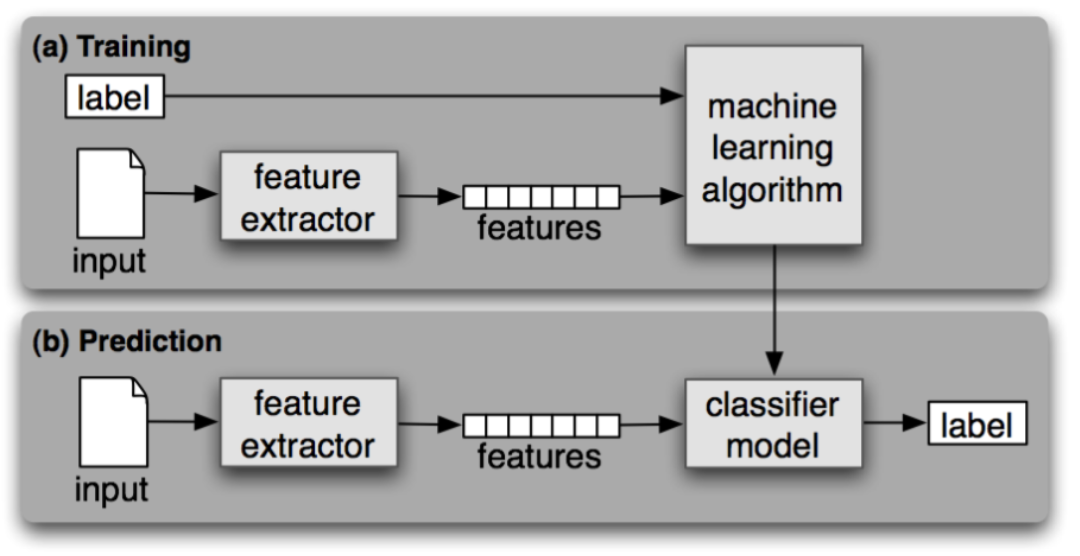
\includegraphics[scale = .3]{images/sentiment_analysis/automatic_systems.png}
      \caption{Training and Prediction Process of Automatic Systems for Sentiment Analysis}
      \label{simulationfigure}
  \end{figure}

During the training process of automatic systems, the textual data is considered as the input while the sentiment labels (positive, negative, or neutral) are considered as labels. The labels and textual data is split into a training and test set in order to check for overfitting after the model has been created. The textual data is based through the feature extractor before being fed into the machine learning algorithm. The feature extractor executes the text preprocessing tasks by cleaning the textual dataset and using text to vector conversion. Once the training dataset is in vector format, it is fed into the machine learning classification algorithm along with its respective labels. After the model is trained, we use the test dataset to check the performance of our machine learning algorithm. Checking our model with a test dataset helps us make sure that our model is generalizable and not overfitting to our training dataset. Once a suitable model has been developed, we can use it to predict the labels of new unstructured textual data. Once the new text, that does not contain a sentiment label, has been projected onto a vector space, we can feed it into our model to get a suitable prediction about the sentiment of the document. Deep learning automatic systems work best for sentiment analysis if provided with huge training and test datasets. Most people do not train their own automatic systems for sentiment analysis as it is very time consuming and costly to develop a pre labeled textual dataset. Instead most of the automatic systems used today are pre trained by large data science and Artificial Intelligence corporations.

  \item \emph{Hybrid} systems combine both the rule based and automatic approaches. Hybrid systems can gain higher precession and accuracy by combining the best of both worlds.

\end{itemize}

\subsubsection{Models for Sentiment Analysis}

In this section, I am going to discuss the models that I used for sentiment analysis on the news articles dataset. A combination of rule based and automatic sentiment analysis systems are used in an effort to identify the best sentiment extraction technique for predicting short run directional change in exchange rates. Following is the list of sentiment analysis techniques that were used:

\begin{itemize}
  \item \emph{Tonality Dictionary} is a rule based system with 231 positive words and 102 negative words in its dictionary. The sentiment analysis model is a reconstruction of the model used in the paper 'What's the Story? A New Perspective on the Value of Economic Forecasts' where the author uses it to measure the degree of optimism and pessimism regarding Federal Reserve Board forecasts published in the Greenbook. I developed the same model in Python for conducting sentiment analysis on foreign exchange news articles using the paper's positive and negative words dictionary along with tf-idf weighting scheme.

  \item \emph{VADER} stands for Valence Aware Dictionary and sEntiment Reasonser. It is an open source pre-trained algorithm that works based of a simple rule based model for conducting sentiment analysis. It was created and optimized to sentiments expressed on social media like twitter, online news, movie/product reviews etc. Furthermore, VADER is also able to include sentiments for emoticons (e.g. :D), acronyms (e.g. LoL) and slang. I decided to use VADER for sentiment analysis on FOREX news articles because of its reputation for performing well on online media including news articles. The compound score in VADER's result is an aggregate of negative, positive and neutral sentiment score of a text. If the compound score of a document is greater than or equal to 0.05, it is considered to be positive. On the other hand, If the compound score of a document is less than or equal to -0.05, it is considered to be negative. Anything between -0.05 to 0.05 indicates a neutral sentiment.

  \item \emph{TextBlob} is a python package that can be used for sentiment analysis. It is a rule based system that works well with negation and modifier words. This means that it is able to classify 'great' as positive while 'not great' as negative. It also understands modifiers which means that it will assign a higher positive sentiment score to 'very great' than 'great'. It ignores one letter words in its sentiment phrases which means that sentences like 'not a very great' will be assigned the same negative sentiment score as 'not very great.' Lastly, it also ignores any words it does not know anything about. This means that it will assign the same negative sentiment score to 'not a very great calculation' as it will to 'not a very great'. I decided to use it as one of my models for sentiment analysis because of its understanding of different text structure that play a role in sentiment extraction. A sentiment score that is greater than 0 is considered to be positive while anything less than 0 is considered negative. A score of exactly 0 is considered to be neutral(which is rarely the case in documents.)

  \item \emph{Harvard IV-4 Dictionary} is a dictionary developed by Harvard University that can be used for sentiment analysis. It contains a list of positive and negative words according to the psychological Harvard IV-4 dictionary as used in general inquirer software. It is one of the most widely used dictionaries for sentiment analysis. I used the dictionary to develop a rule based system that assigns a score of greater then 0 for positive sentiment, a score of less than 0 for negative sentiment, and a score of 0 for neutral sentiment.

  \item \emph{Loughran and Mcdonald (LM) Dictionary} is a dictionary developed specifically for the accounting and financial domain. According to the Loughran and McDonald (2011) article, applying a general sentiment word list to accounting and financial documents can lead to high rate of misclassification. It is for this reason that they developed a custom positive and negative words financial dictionary. They also added an \emph{uncertainity} word list that attempts to measure the general notion of imprecision. The financial dictionary contains 2339 negative words and 353 positive words. I used the dictionary to develop a rule based system that assigns a score of greater then 0 for positive sentiment, a score of less than 0 for negative sentiment, and a score of 0 for neutral sentiment.

  \item \emph{Aggregate Sentiment} system determines the sentiment of an article by averaging the sentiment score of all five models discussed above. The aggregate sentiment systems is an ensemble method that aims to tap into the strengths of all previous models. \emph{Ensemble methods} are meta-algorithms that combine different machine learning techniques into an overall model that aims to reduce variance , bias or improve predictions. The aggregate model was developed based on the hypothesis that a combination of our models will perform better than one specific model. It will assign a positive sentiment score to any document that has been classified as positive by 3 or more of our sentiment algorithms out of the 5 total systems. Likewise, any document that has been classified as negative by 3 or more of our sentiment algorithms will be given a negative sentiment tag. The same condition holds for assigning neutral sentiment to a piece of text.

\end{itemize}

\newpage

\subsubsection{Results}

This section shows the accuracy of different sentiment models in predicting the directional change in exchange rates at varying lagged intervals. A binary variable for directional change in exchange rate is created. A positive percentage change in exchange rate is given a value of 1, while a negative percentage change in exchange rate is given a value of 0. Lags for the directional change in exchange rate are in daily frequency ranging from 0 to 30. A lag to 0 checks for whether a sentiment model can predict the same day directional change in exchange rate, while a lag of 30 checks for whether a model can predict one month ahead directional change in exchange rate.The number of accurate predictions of the sentiment model is calculated by adding up the number of times the lagged directional change in exchange rates is same as the sentiment score predicted by the model. Afterwards, the accuracy percentage of the model is calculated by dividing the number of accurate predictions by the total length of the dataset and multiplying the answer by 100. The figures below show the accuracy results of all are sentiment models for all currencies in our dataset:


\begin{figure}[H]
    \centering
    \hspace*{-1.8in}
    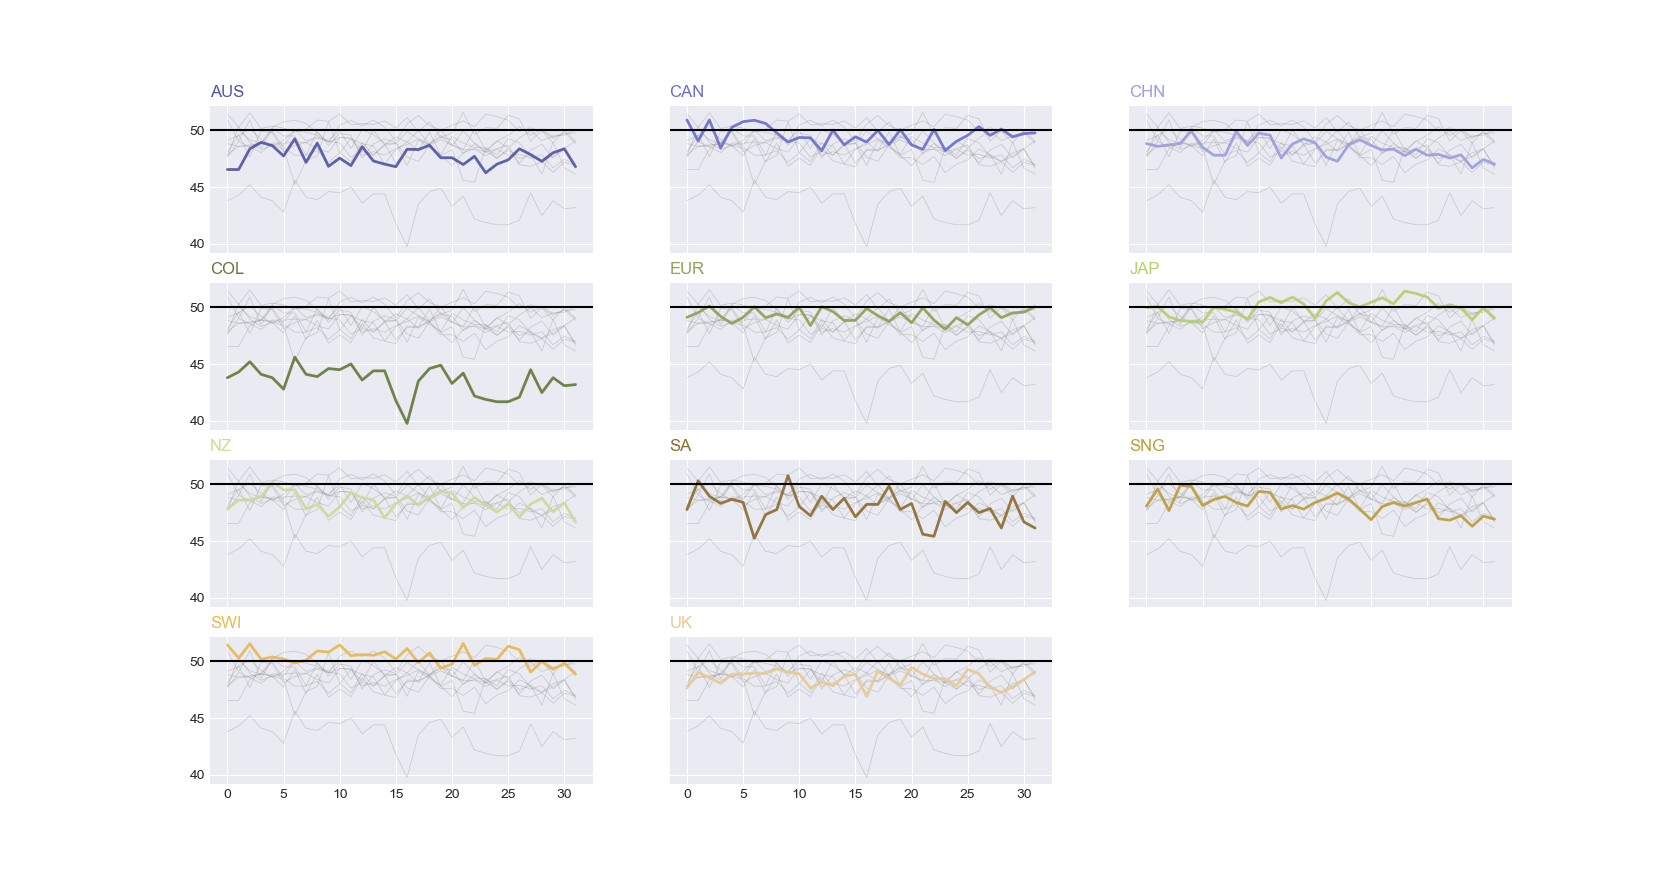
\includegraphics[scale = .5]{images/sentiment_analysis/manual_score.png}
    \caption{Accuracy of Tonality Dictionary Model at Varying Intervals}
    \label{simulationfigure}
\end{figure}

\begin{figure}[H]
    \centering
    \vspace*{-1.3in}
    \hspace*{-1.8in}
    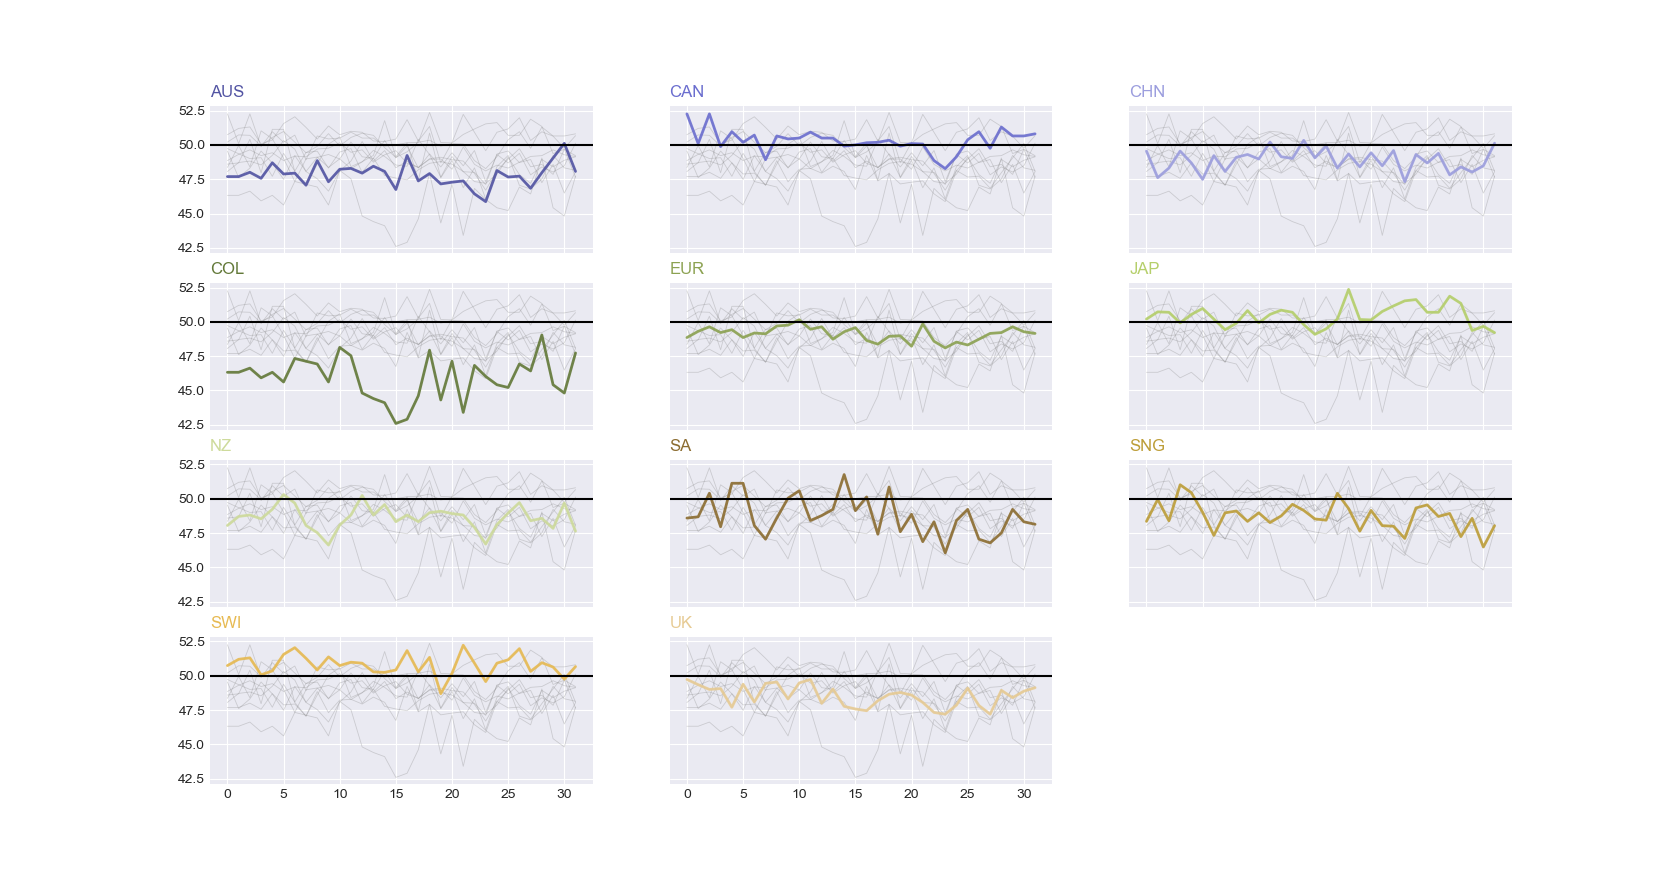
\includegraphics[scale = .46]{images/sentiment_analysis/vader_score.png}
    \caption{Accuracy of VADER Model at Varying Intervals}
    \label{simulationfigure}
\end{figure}

\begin{figure}[H]
    \centering
    \vspace*{-0.2in}
    \hspace*{-1.8in}
    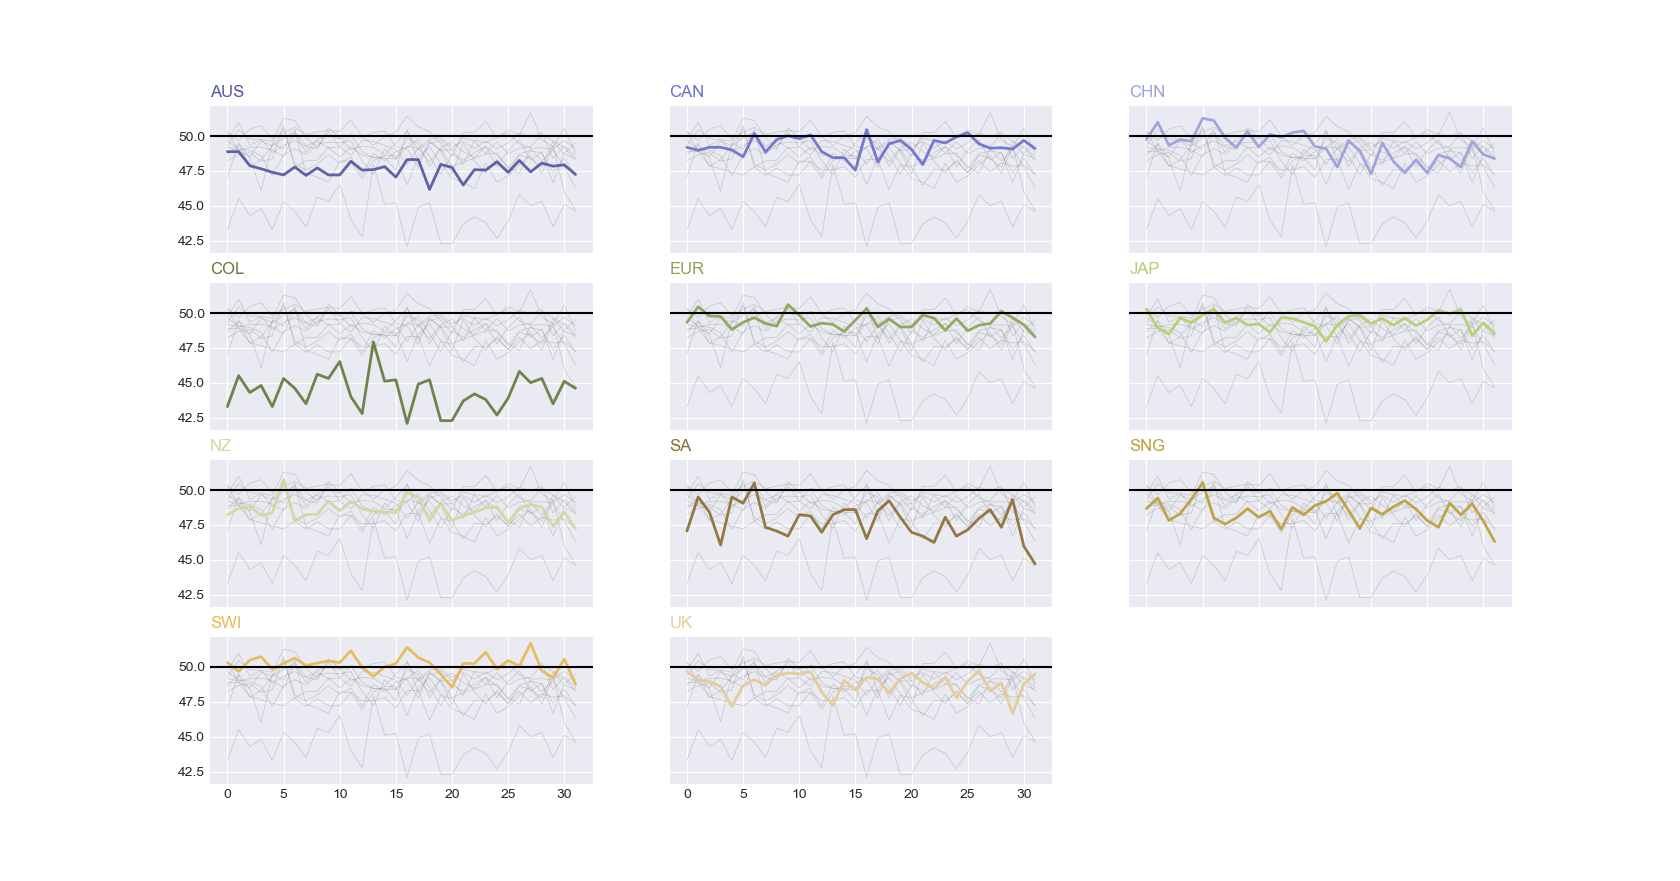
\includegraphics[scale = .46]{images/sentiment_analysis/textblob_score.png}
    \caption{Accuracy of Text Blob Model at Varying Intervals}
    \label{simulationfigure}
\end{figure}

\begin{figure}[H]
    \centering
    \vspace*{-1.3in}
    \hspace*{-1.8in}
    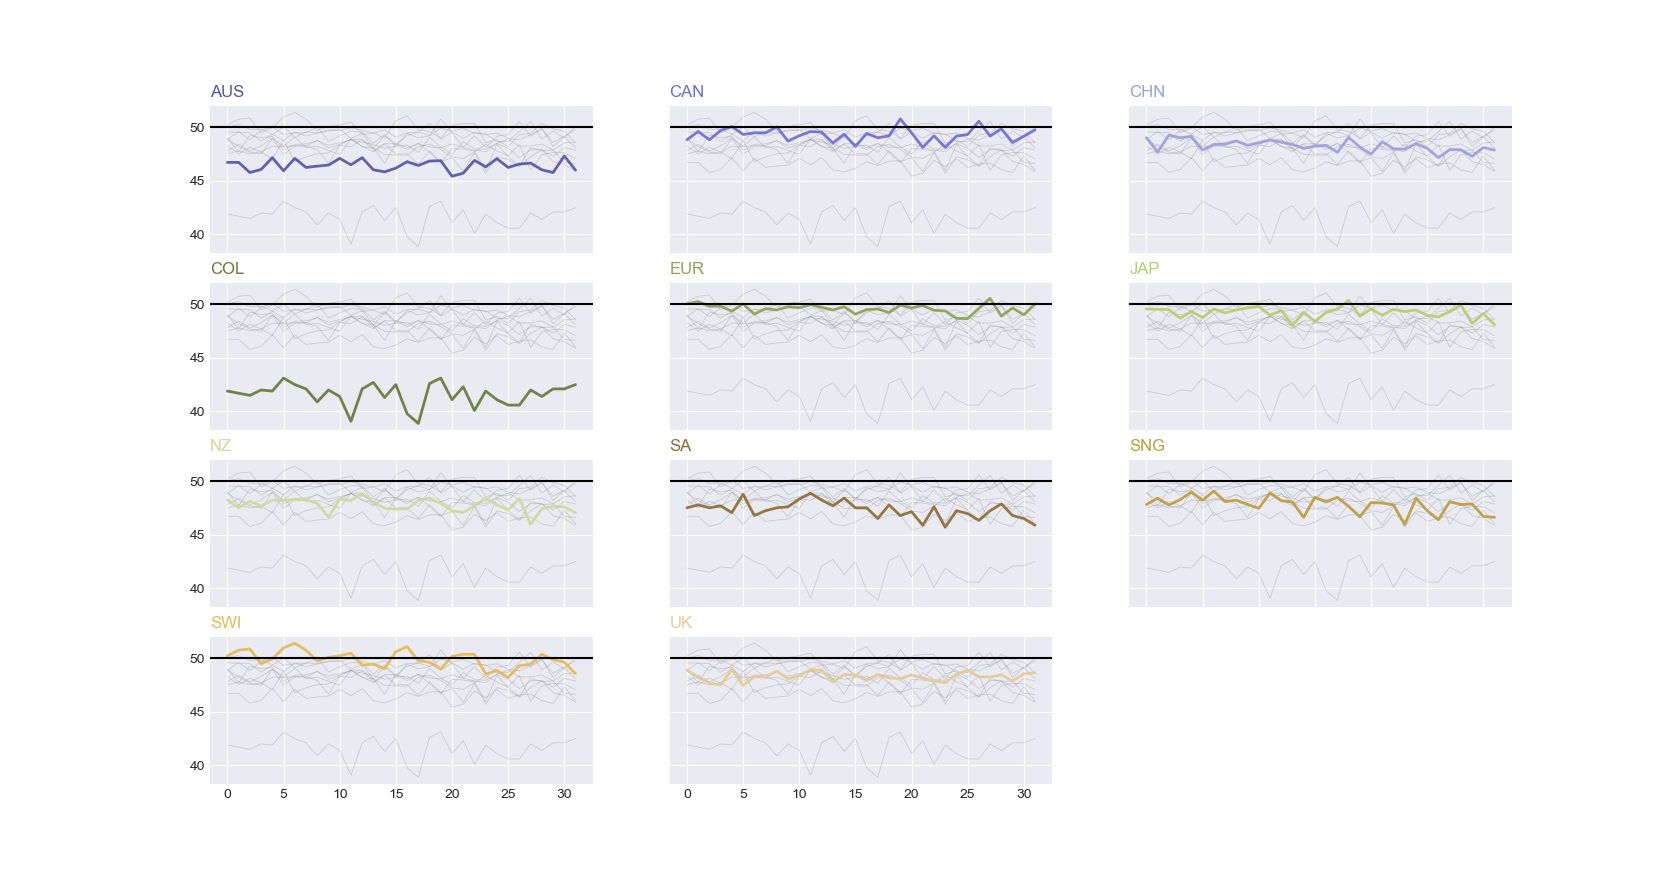
\includegraphics[scale = .46]{images/sentiment_analysis/hiv4_score.png}
    \caption{Accuracy of Harvard IV-4 Dictionary Model at Varying Intervals}
    \label{simulationfigure}
\end{figure}

\begin{figure}[H]
    \centering
    \vspace*{-0.2in}
    \hspace*{-1.8in}
    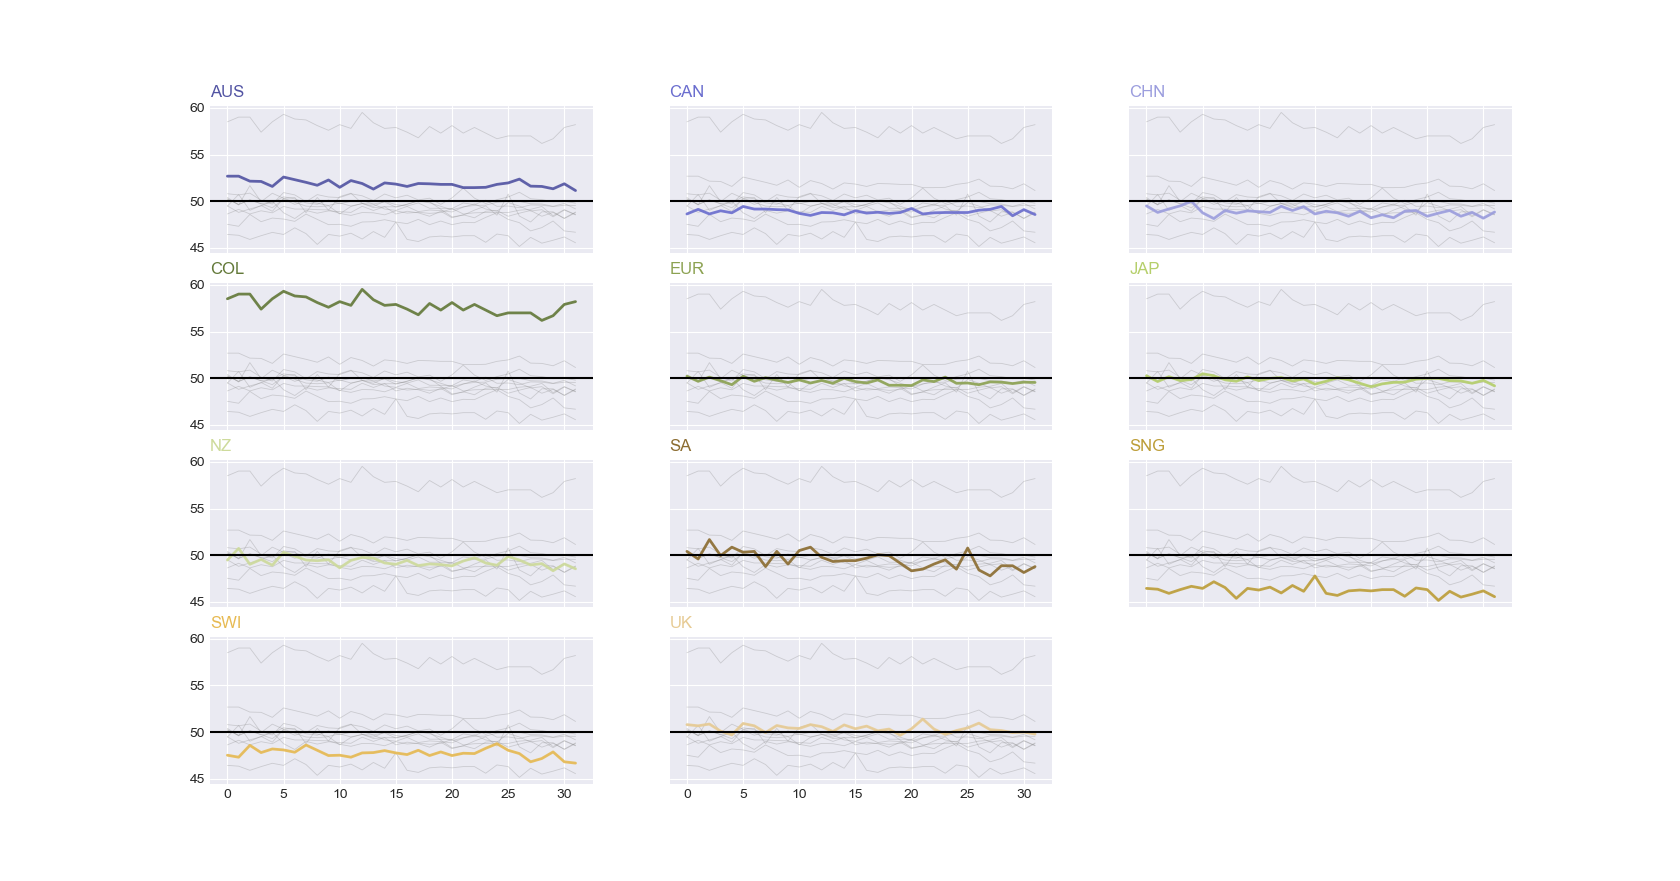
\includegraphics[scale = .46]{images/sentiment_analysis/lm_score.png}
    \caption{Accuracy of LM Dictionary Model at Varying Intervals}
    \label{simulationfigure}
\end{figure}

\begin{figure}[H]
    \centering
    \hspace*{-1.8in}
    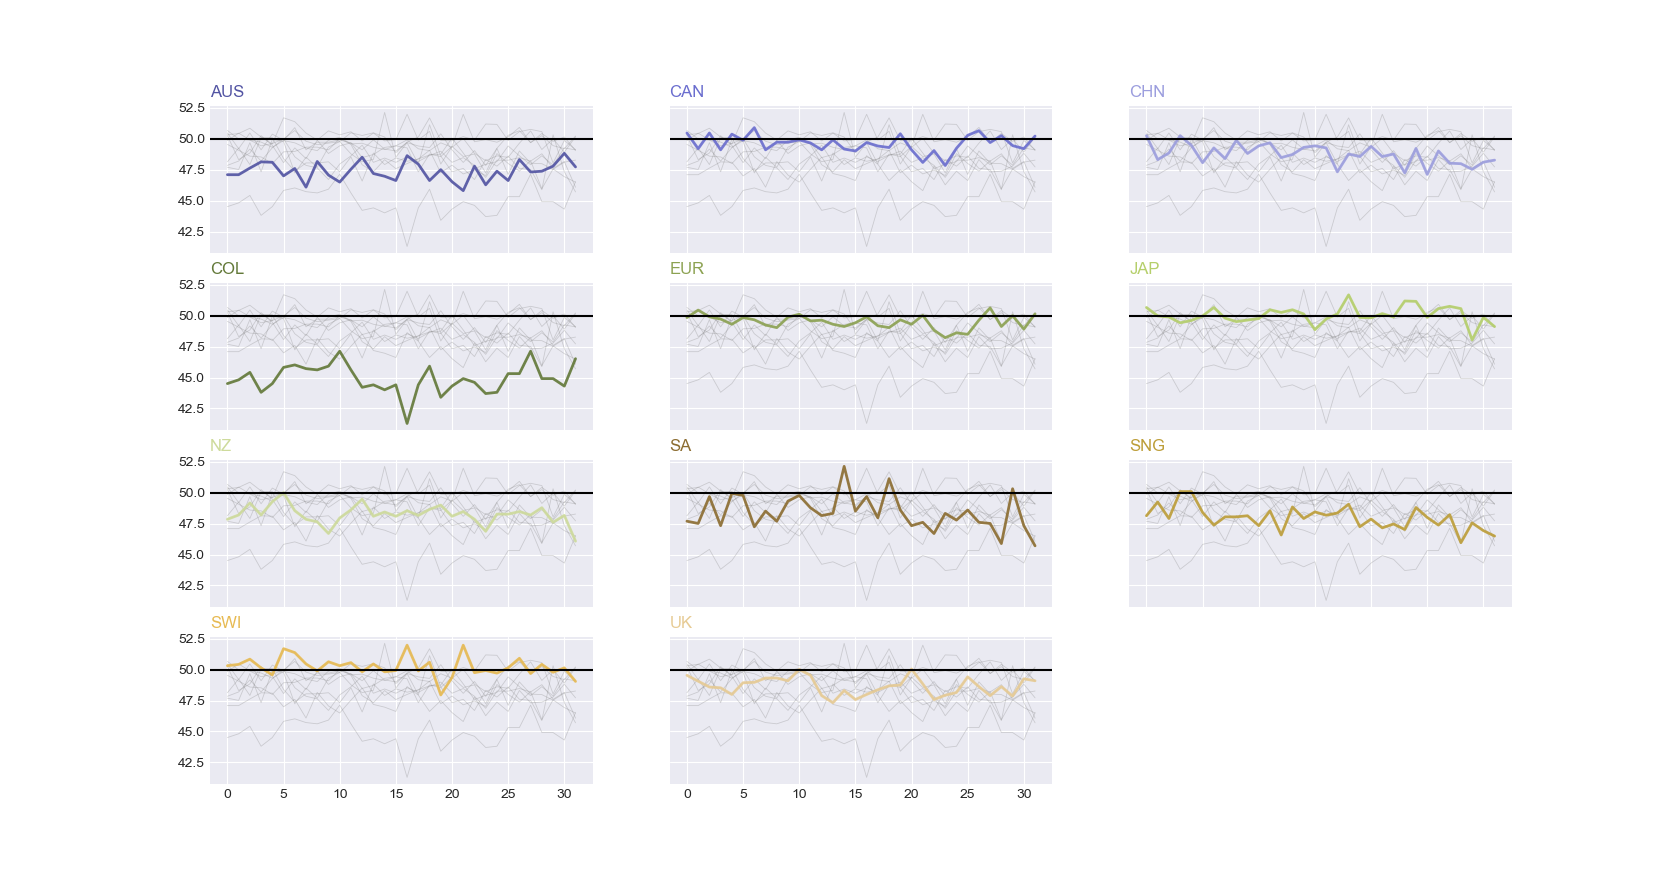
\includegraphics[scale = .5]{images/sentiment_analysis/aggregate_score.png}
    \caption{Accuracy of Aggregate Model at Varying Intervals}
    \label{simulationfigure}
\end{figure}

\begin{itemize}
  \item Different models seem to perform better for different countries. It is interesting to see how most of our models get their lowest accuracy score when trying to predict directional change in Colombia's exchange rate. While, the Loughran and Mcdonald dictionary model, on the other hand, appears to predict Colombia's directional exchange rate with a drastically high accuracy of 60 percent.

  \item There seems to be no set relationship between the lagged interval for directional change in exchange rate and the accuracy score. Different models seem to perform better for different countries at varying lag intervals. For some countries, a model might perform well over a small lag value, while for others the same model might perform better over a larger lag value.

  \item Combining sentiment model results into one aggregate model does not seem to significantly improve its accuracy. This might be because all models are given similar weight while aggregating the sentiment results. Introducing some form of dynamic weighting mechanism into the aggregating model might improve the accuracy of the model.

  \item Different models seem to outperform the random walk model for different countries at varying lagged intervals. On average, the sentiment analysis models do not seem to perform better than the random walk model. This might be because of the ineffectiveness of the sorting text algorithm that we used to divide news paper articles by country. Developing a better sorting mechanism for distribution articles as per country might drastically improve the efficiency of our models.
\end{itemize}



\end{document}
